\chapter{More UK Biobank results}\label{appendix:more-ukb-results}
%%%%%

%%
\section{Results for other depression phenotypes}\label{appendix:more-ukb-results-other-phenotypes}
%%


\begin{figure}[ht]
  \centering
  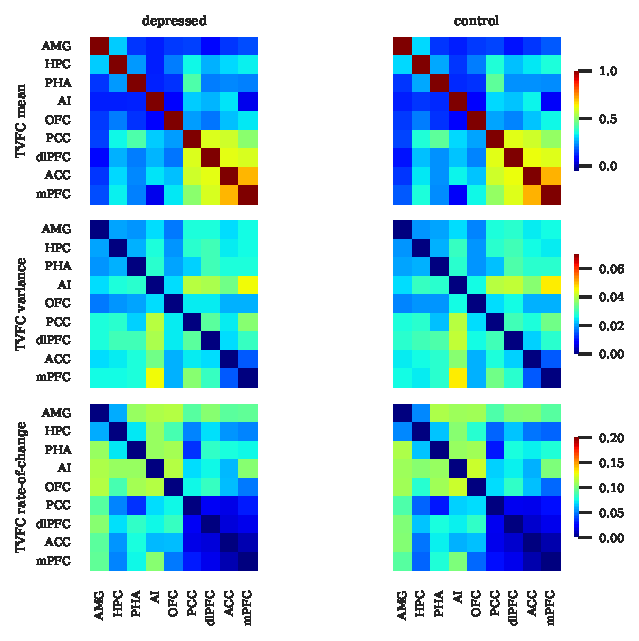
\includegraphics[width=0.9\textwidth]{fig/ukbiobank/TVFC_predictions_summaries/lifetime_occurrence/cohort_comparison/ROI/correlation_TVFC_estimates_SVWP_joint_joint}
  \caption{
    Self-reported depression lifetime occurrence analysis - SVWP estimates.
    Mean over 808 subjects per cohort for all ROI edges, for three TVFC summary measures.
  }\label{fig:ukb-results-lo-roi-cohort-comparison-full-wp}
\end{figure}


\begin{figure}[ht]
  \centering
  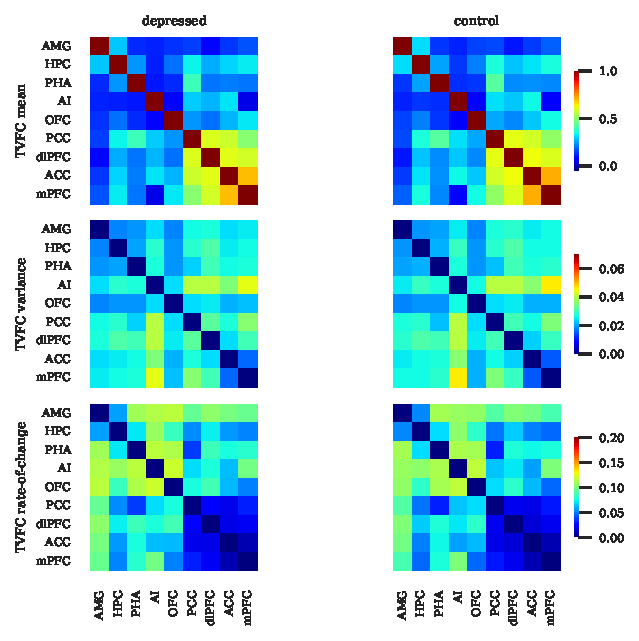
\includegraphics[width=0.9\textwidth]{fig/ukbiobank/TVFC_predictions_summaries/self_reported_depression_state/cohort_comparison/ROI/correlation_TVFC_estimates_SVWP_joint_joint}
  \caption{
    Self-reported depressed state analysis - SVWP estimates.
    Mean over 1,411 subjects per cohort for all ROI edges, for three TVFC summary measures.
  }\label{fig:ukb-results-srds-roi-cohort-comparison-full-wp}
\end{figure}


\begin{figure}[ht]
    \centering
    \subcaptionbox{High | TVFC mean\label{fig:ukb-results-pgs-cohort-comparison-full-wp-mean-high}}{\includegraphics[width=0.32\textwidth]{fig/ukbiobank/TVFC_predictions_summaries/pgs/pgs_high/ROI/correlation_TVFC_mean_SVWP_joint}}
    \subcaptionbox{Med | TVFC mean\label{fig:ukb-results-pgs-cohort-comparison-full-wp-mean-med}}{\includegraphics[width=0.32\textwidth]{fig/ukbiobank/TVFC_predictions_summaries/pgs/pgs_medium/ROI/correlation_TVFC_mean_SVWP_joint}}
    \subcaptionbox{Low | TVFC mean\label{fig:ukb-results-pgs-cohort-comparison-full-wp-mean-low}}{\includegraphics[width=0.32\textwidth]{fig/ukbiobank/TVFC_predictions_summaries/pgs/pgs_low/ROI/correlation_TVFC_mean_SVWP_joint}}
    \subcaptionbox{High | TVFC variance\label{fig:ukb-results-pgs-cohort-comparison-full-wp-var-high}}{\includegraphics[width=0.32\textwidth]{fig/ukbiobank/TVFC_predictions_summaries/pgs/pgs_high/ROI/correlation_TVFC_variance_SVWP_joint}}
    \subcaptionbox{Med | TVFC variance\label{fig:ukb-results-pgs-cohort-comparison-full-wp-var-med}}{\includegraphics[width=0.32\textwidth]{fig/ukbiobank/TVFC_predictions_summaries/pgs/pgs_medium/ROI/correlation_TVFC_variance_SVWP_joint}}
    \subcaptionbox{Low | TVFC variance\label{fig:ukb-results-pgs-cohort-comparison-full-wp-var-low}}{\includegraphics[width=0.32\textwidth]{fig/ukbiobank/TVFC_predictions_summaries/pgs/pgs_low/ROI/correlation_TVFC_variance_SVWP_joint}}
    \subcaptionbox{High | TVFC rate-of-change\label{fig:ukb-results-pgs-cohort-comparison-full-wp-roc-high}}{\includegraphics[width=0.32\textwidth]{fig/ukbiobank/TVFC_predictions_summaries/pgs/pgs_high/ROI/correlation_TVFC_rate_of_change_SVWP_joint}}
    \subcaptionbox{Med | TVFC rate-of-change\label{fig:ukb-results-pgs-cohort-comparison-full-wp-roc-med}}{\includegraphics[width=0.32\textwidth]{fig/ukbiobank/TVFC_predictions_summaries/pgs/pgs_medium/ROI/correlation_TVFC_rate_of_change_SVWP_joint}}
    \subcaptionbox{Low | TVFC rate-of-change\label{fig:ukb-results-pgs-cohort-comparison-full-wp-roc-low}}{\includegraphics[width=0.32\textwidth]{fig/ukbiobank/TVFC_predictions_summaries/pgs/pgs_low/ROI/correlation_TVFC_rate_of_change_SVWP_joint}}
    \caption{
        Polygenic risk scores analysis - SVWP estimates.
        Mean over 3,775 subjects per cohort for all ROI edges, for three TVFC summary measures.
    }\label{fig:ukb-results-pgs-roi-cohort-comparison-full-wp}
\end{figure}


%%
\clearpage
\section{Results with other TVFC estimation methods}\label{appendix:more-ukb-results-other-tvfc-methods}
%%

%%
\clearpage
\subsection{Diagnosed lifetime occurrence - ROI analysis}
%%


\begin{figure}[h]
  \centering
  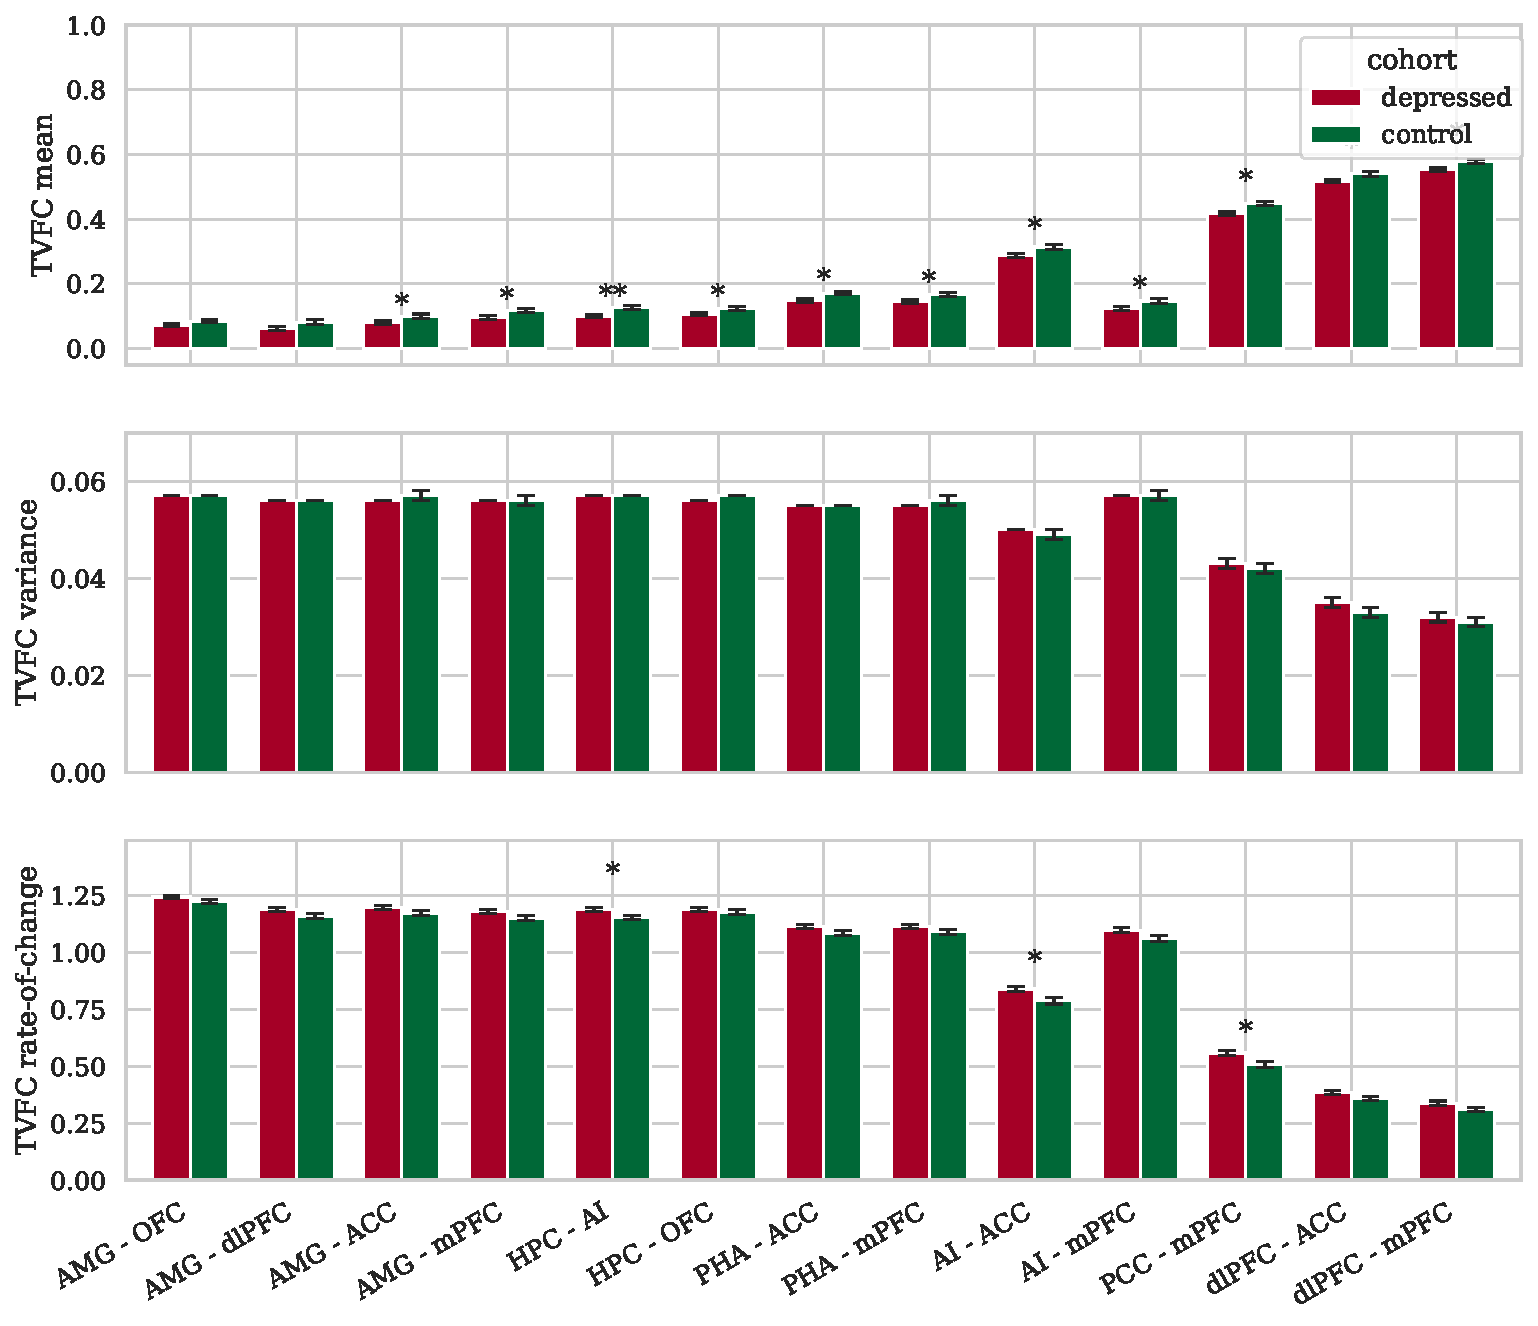
\includegraphics[width=\textwidth]{fig/ukbiobank/TVFC_predictions_summaries/diagnosed_lifetime_occurrence/cohort_comparison/ROI/correlation_all_TVFC_summary_measures_DCC_joint_edges_of_interest}
  \caption{
    Diagnosed depression lifetime occurrence analysis - brain regions of interest - DCC (joint) estimates.
    Mean and standard error over 620 subjects per cohort for edges of interest for three TVFC summary measures.
    *: $p \leq .05$, **: $p \leq .01$.
  }\label{fig:ukb-results-dlo-roi-cohort-comparison-edges-of-interest-dcc-j}
\end{figure}


\begin{figure}[h]
    \centering
    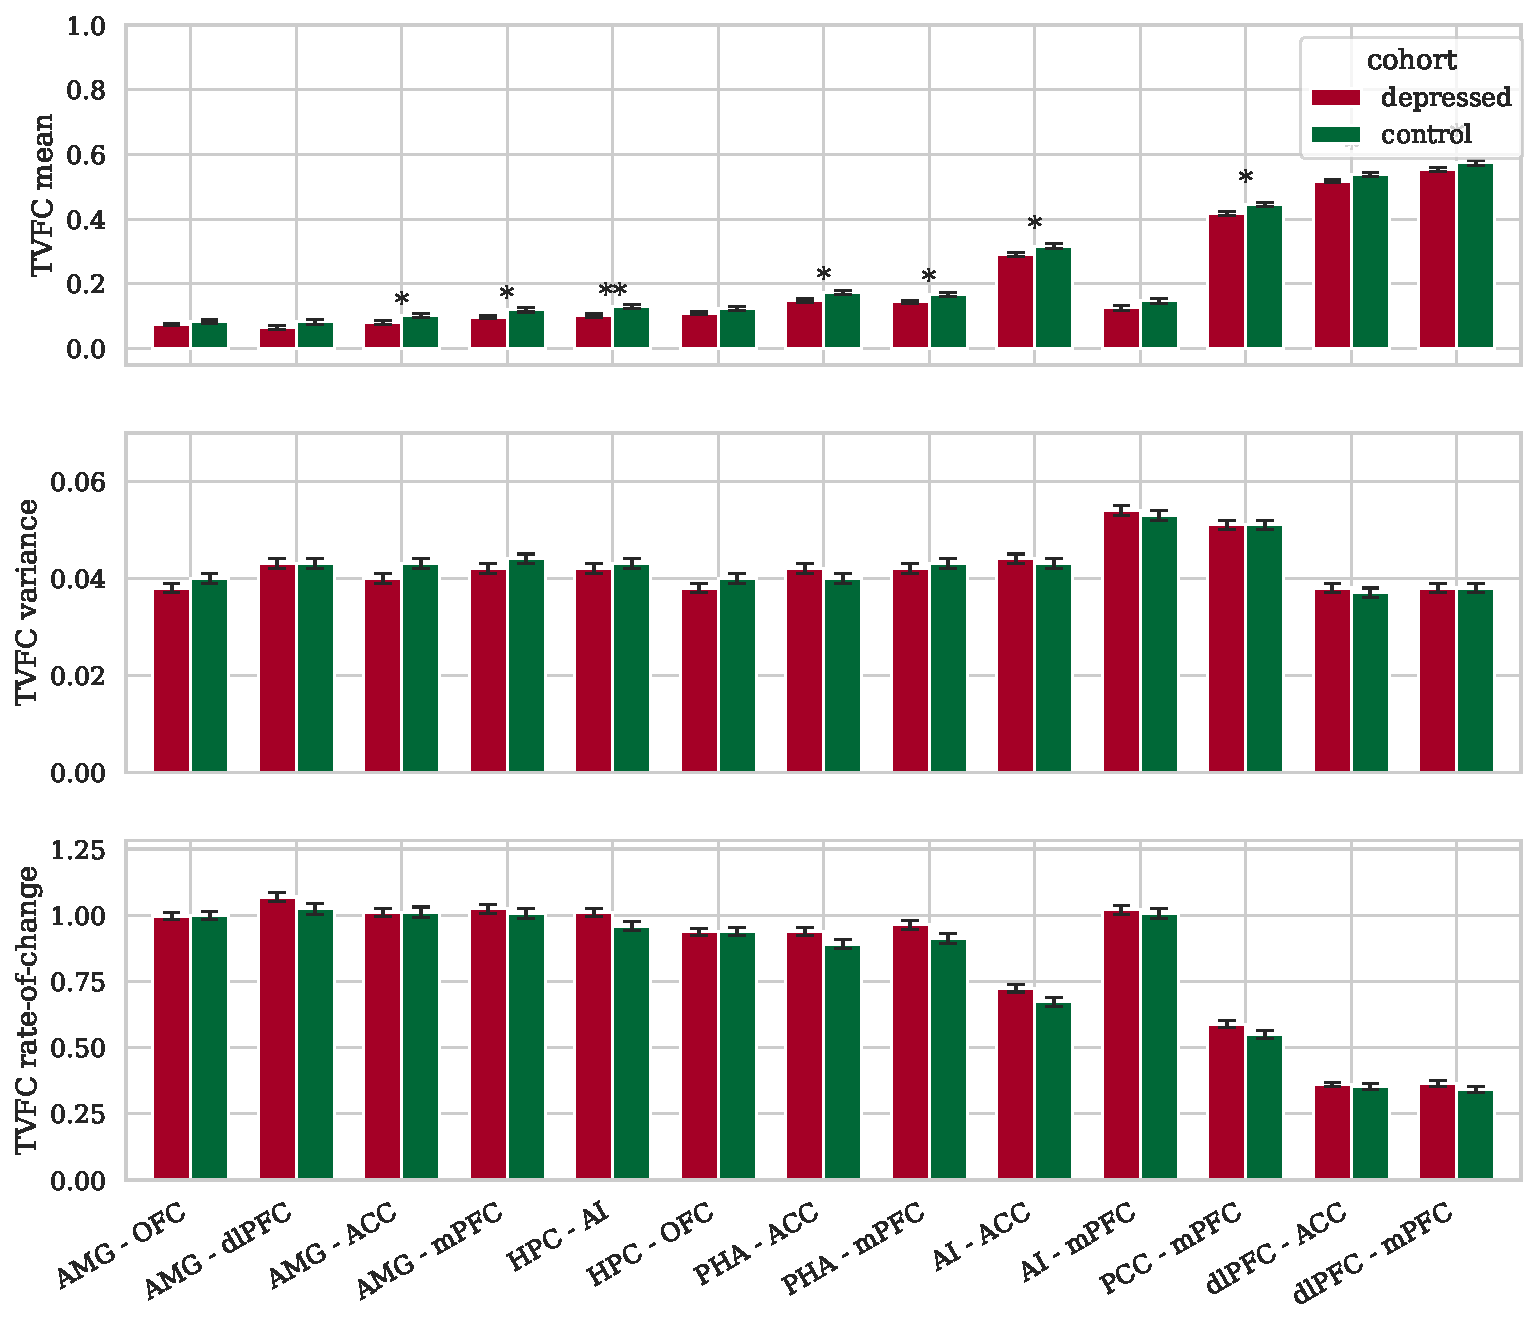
\includegraphics[width=\textwidth]{fig/ukbiobank/TVFC_predictions_summaries/diagnosed_lifetime_occurrence/cohort_comparison/ROI/correlation_all_TVFC_summary_measures_DCC_bivariate_loop_edges_of_interest}
    \caption{
        Diagnosed depression lifetime occurrence analysis - brain regions of interest - DCC (bivariate loop) estimates.
        Mean and standard error over 620 subjects per cohort for edges of interest for three TVFC summary measures.
        *: $p \leq .05$, **: $p \leq .01$.
    }\label{fig:ukb-results-dlo-roi-cohort-comparison-edges-of-interest-dcc-bl}
\end{figure}


\begin{figure}[h]
    \centering
    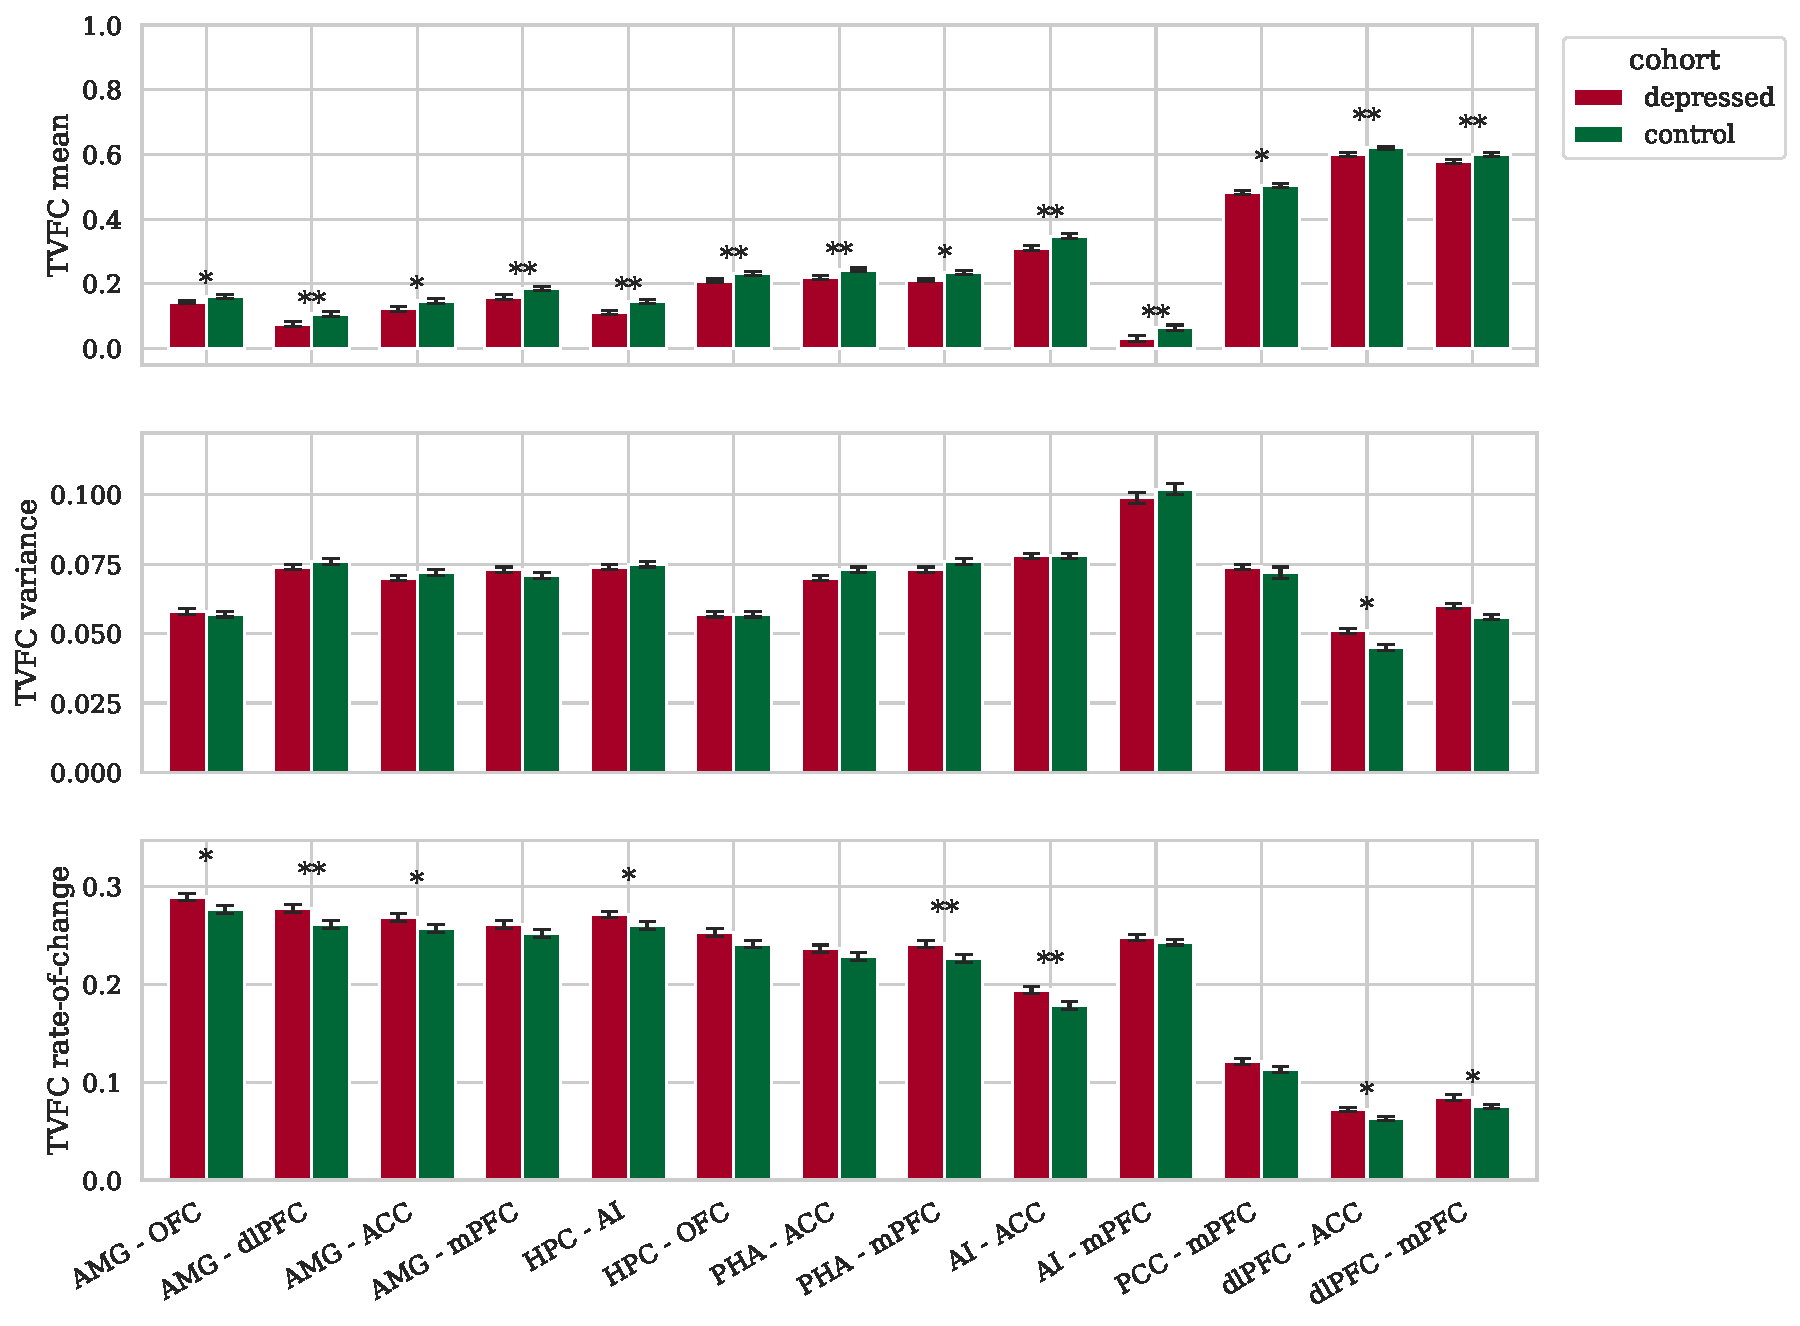
\includegraphics[width=\textwidth]{fig/ukbiobank/TVFC_predictions_summaries/diagnosed_lifetime_occurrence/cohort_comparison/ROI/correlation_all_TVFC_summary_measures_SW_cross_validated_edges_of_interest}
    \caption{
        Diagnosed depression lifetime occurrence analysis - brain regions of interest - SW-CV estimates.
        Mean and standard error over 620 subjects per cohort for edges of interest for three TVFC summary measures.
        *: $p \leq .05$, **: $p \leq .01$.
    }\label{fig:ukb-results-dlo-roi-cohort-comparison-edges-of-interest-sw-cv}
\end{figure}


\begin{figure}[h]
    \centering
    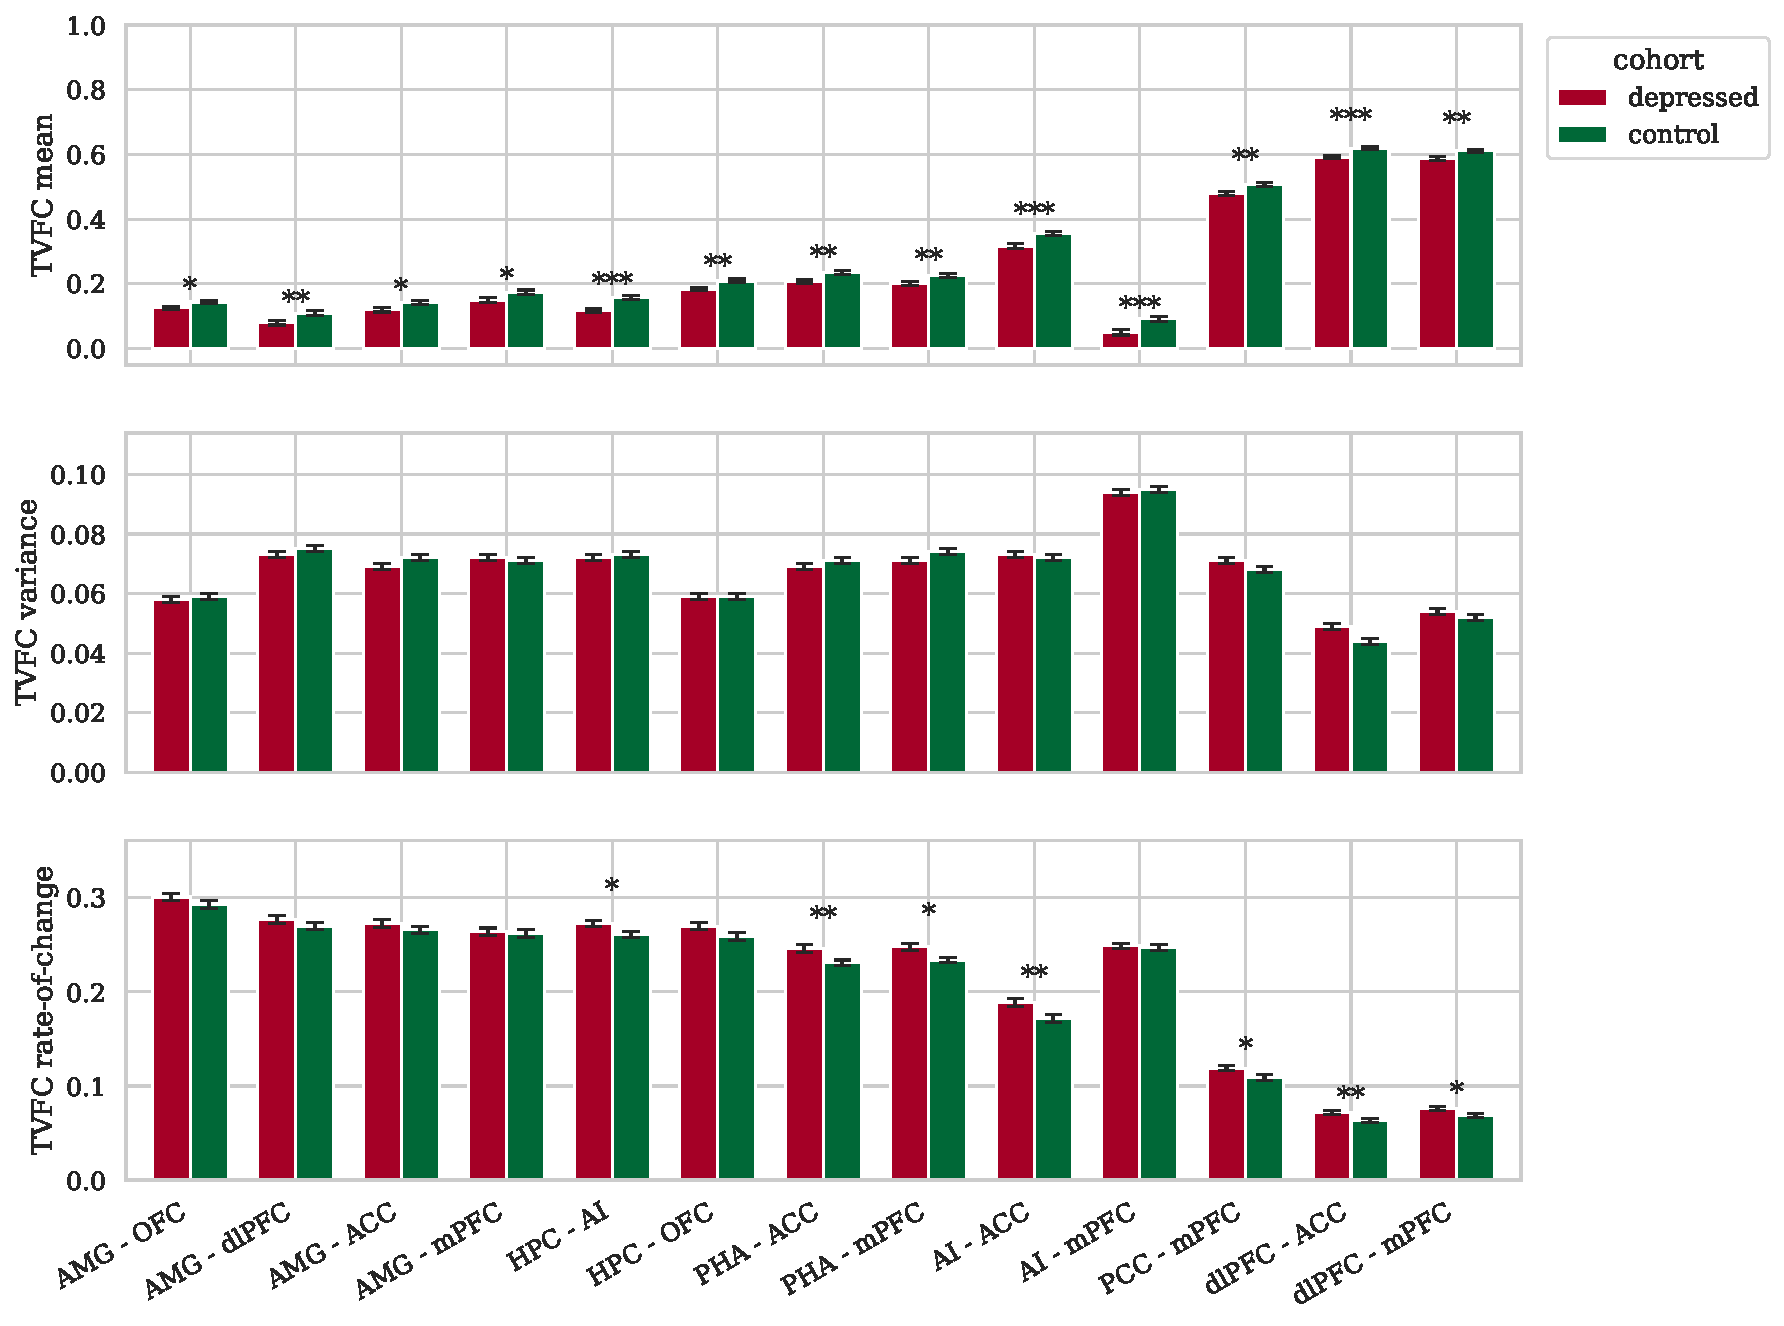
\includegraphics[width=\textwidth]{fig/ukbiobank/TVFC_predictions_summaries/diagnosed_lifetime_occurrence/cohort_comparison/ROI/correlation_all_TVFC_summary_measures_SW_30_edges_of_interest}
    \caption{
        Diagnosed depression lifetime occurrence analysis - brain regions of interest - SW (30 seconds window) estimates.
        Mean and standard error over 620 subjects per cohort for edges of interest for three TVFC summary measures.
        *: $p \leq .05$, **: $p \leq .01$.
    }\label{fig:ukb-results-dlo-roi-cohort-comparison-edges-of-interest-sw-30}
\end{figure}


\begin{figure}[h]
    \centering
    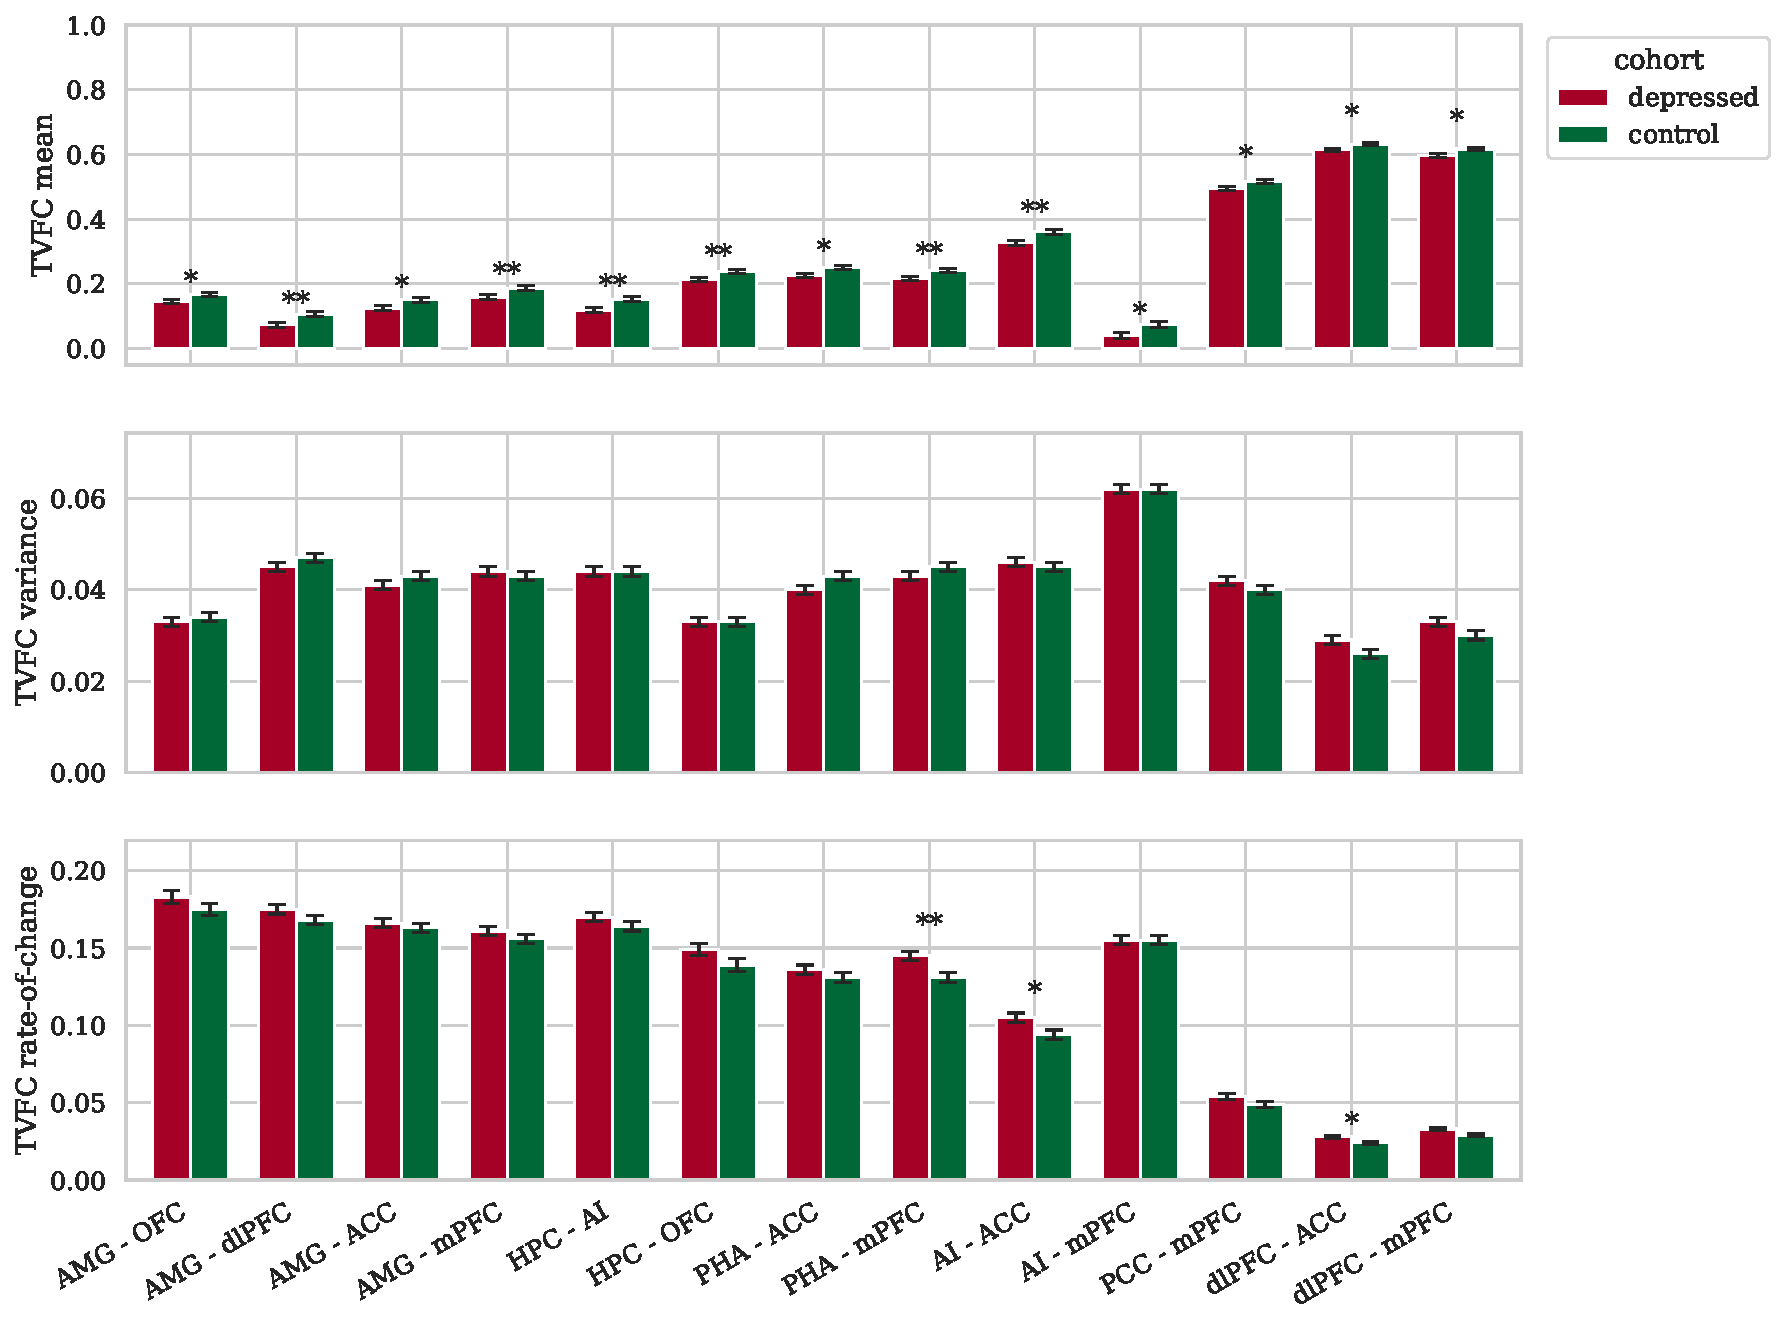
\includegraphics[width=\textwidth]{fig/ukbiobank/TVFC_predictions_summaries/diagnosed_lifetime_occurrence/cohort_comparison/ROI/correlation_all_TVFC_summary_measures_SW_60_edges_of_interest}
    \caption{
        Diagnosed depression lifetime occurrence analysis - brain regions of interest - SW (60 seconds window) estimates.
        Mean and standard error over 620 subjects per cohort for edges of interest for three TVFC summary measures.
        *: $p \leq .05$, **: $p \leq .01$.
    }\label{fig:ukb-results-dlo-roi-cohort-comparison-edges-of-interest-sw-60}
\end{figure}


%%
\clearpage
\subsection{Diagnosed lifetime occurrence - FN analysis}
%%


\begin{figure}[h]
  \centering
  \includegraphics[width=0.7\textwidth]{fig/ukbiobank/TVFC_predictions_summaries/diagnosed_lifetime_occurrence/cohort_comparison/FN/correlation_all_TVFC_summary_measures_DCC_joint_edges_of_interest}
  \caption{
    Diagnosed depression lifetime occurrence analysis - functional networks - DCC (joint) estimates.
    Mean and standard error over 620 subjects per cohort for edges of interest for three TVFC summary measures.
    *: $p \leq .05$, **: $p \leq .01$, ***: $p \leq .001$.
  }\label{fig:ukb-results-dlo-fn-cohort-comparison-edges-of-interest-dcc-j}
\end{figure}


\begin{figure}[h]
    \centering
    \includegraphics[width=0.7\textwidth]{fig/ukbiobank/TVFC_predictions_summaries/diagnosed_lifetime_occurrence/cohort_comparison/FN/correlation_all_TVFC_summary_measures_DCC_bivariate_loop_edges_of_interest}
    \caption{
        Diagnosed depression lifetime occurrence analysis - functional networks - DCC (bivariate loop) estimates.
        Mean and standard error over 620 subjects per cohort for edges of interest for three TVFC summary measures.
        *: $p \leq .05$, **: $p \leq .01$, ***: $p \leq .001$.
    }\label{fig:ukb-results-dlo-fn-cohort-comparison-edges-of-interest-dcc-bl}
\end{figure}


\begin{figure}[h]
    \centering
    \includegraphics[width=0.7\textwidth]{fig/ukbiobank/TVFC_predictions_summaries/diagnosed_lifetime_occurrence/cohort_comparison/FN/correlation_all_TVFC_summary_measures_SW_cross_validated_edges_of_interest}
    \caption{
        Diagnosed depression lifetime occurrence analysis - functional networks - SW-CV estimates.
        Mean and standard error over 620 subjects per cohort for edges of interest for three TVFC summary measures.
        *: $p \leq .05$, **: $p \leq .01$, ***: $p \leq .001$.
    }\label{fig:ukb-results-dlo-fn-cohort-comparison-edges-of-interest-sw-cv}
\end{figure}


\begin{figure}[h]
    \centering
    \includegraphics[width=0.7\textwidth]{fig/ukbiobank/TVFC_predictions_summaries/diagnosed_lifetime_occurrence/cohort_comparison/FN/correlation_all_TVFC_summary_measures_SW_30_edges_of_interest}
    \caption{
        Diagnosed depression lifetime occurrence analysis - functional networks - SW (30 seconds window) estimates.
        Mean and standard error over 620 subjects per cohort for edges of interest for three TVFC summary measures.
        *: $p \leq .05$, **: $p \leq .01$, ***: $p \leq .001$.
    }\label{fig:ukb-results-dlo-fn-cohort-comparison-edges-of-interest-sw-30}
\end{figure}


\begin{figure}[h]
    \centering
    \includegraphics[width=0.7\textwidth]{fig/ukbiobank/TVFC_predictions_summaries/diagnosed_lifetime_occurrence/cohort_comparison/FN/correlation_all_TVFC_summary_measures_SW_60_edges_of_interest}
    \caption{
        Diagnosed depression lifetime occurrence analysis - functional networks - SW (60 seconds window) estimates.
        Mean and standard error over 620 subjects per cohort for edges of interest for three TVFC summary measures.
        *: $p \leq .05$, **: $p \leq .01$, ***: $p \leq .001$.
    }\label{fig:ukb-results-dlo-fn-cohort-comparison-edges-of-interest-sw-60}
\end{figure}



%%%%%%%%%%%%%%%%%%%%%%%%%%%%%%%%%%%%%%%%%%%%%%%%%%%%%%
%%%%%%%%%%%%%%%%%%%%%%%%%%%%%%%%%%%%%%%%%%%%%%%%%%%%%%
%%%%%%%%%%%%%%%%%%%%%%%%%%%%%%%%%%%%%%%%%%%%%%%%%%%%%%
%%%%%%%%%%%%%%%%%%%%%%%%%%%%%%%%%%%%%%%%%%%%%%%%%%%%%%
%%%%%%%%%%%%%%%%%%%%%%%%%%%%%%%%%%%%%%%%%%%%%%%%%%%%%%



%%
\clearpage
\subsection{Self-reported lifetime occurrence - ROI analysis}
%%


\begin{figure}[h]
    \centering
    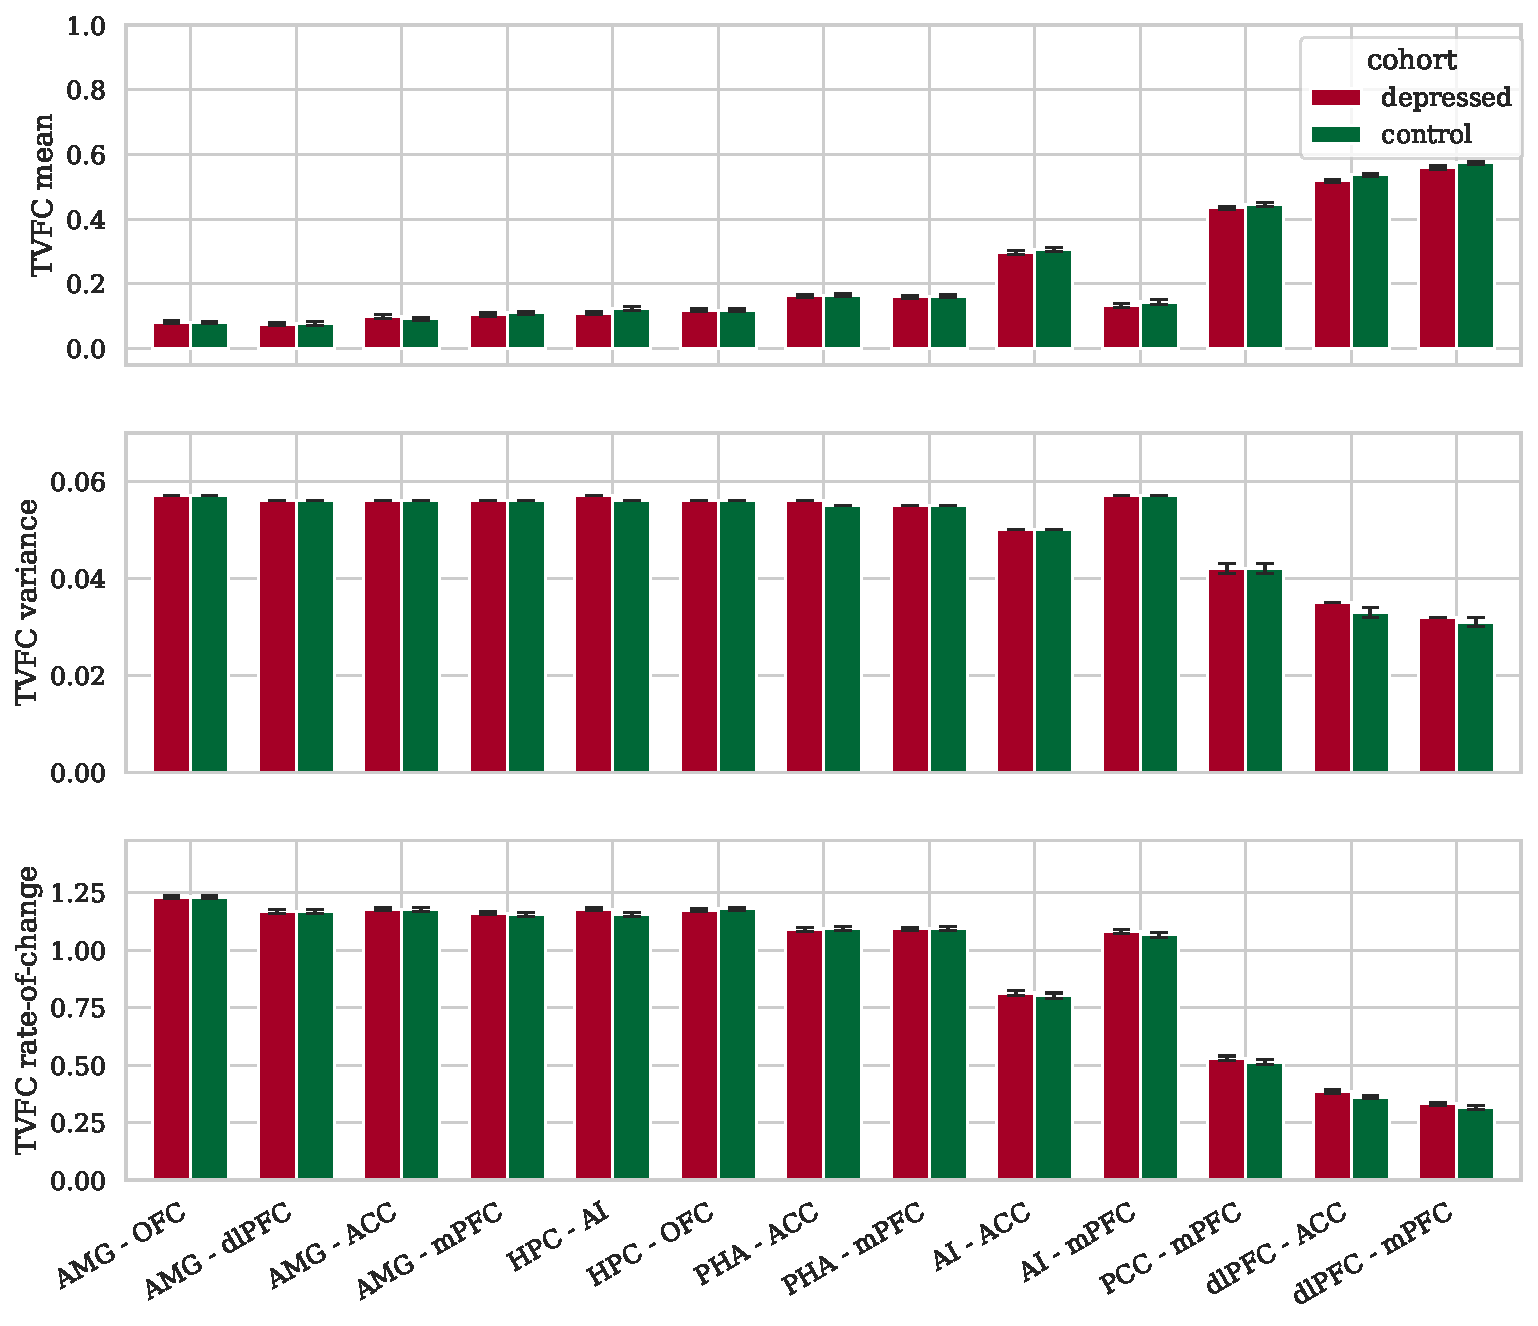
\includegraphics[width=\textwidth]{fig/ukbiobank/TVFC_predictions_summaries/lifetime_occurrence/cohort_comparison/ROI/correlation_all_TVFC_summary_measures_DCC_joint_edges_of_interest}
    \caption{
        Self-reported depression lifetime occurrence analysis - brain regions of interest - DCC (joint) estimates.
        Mean and standard error over 808 subjects per cohort for edges of interest for three TVFC summary measures.
        *: $p \leq .05$.
    }\label{fig:ukb-results-lo-roi-cohort-comparison-edges-of-interest-dcc-j}
\end{figure}


\begin{figure}[h]
    \centering
    \includegraphics[width=\textwidth]{fig/ukbiobank/TVFC_predictions_summaries/lifetime_occurrence/cohort_comparison/ROI/correlation_all_TVFC_summary_measures_DCC_bivariate_loop_edges_of_interest}
    \caption{
        Self-reported depression lifetime occurrence analysis - brain regions of interest - DCC (bivariate loop) estimates.
        Mean and standard error over 808 subjects per cohort for edges of interest for three TVFC summary measures.
        *: $p \leq .05$.
    }\label{fig:ukb-results-lo-roi-cohort-comparison-edges-of-interest-dcc-bl}
\end{figure}


\begin{figure}[h]
    \centering
    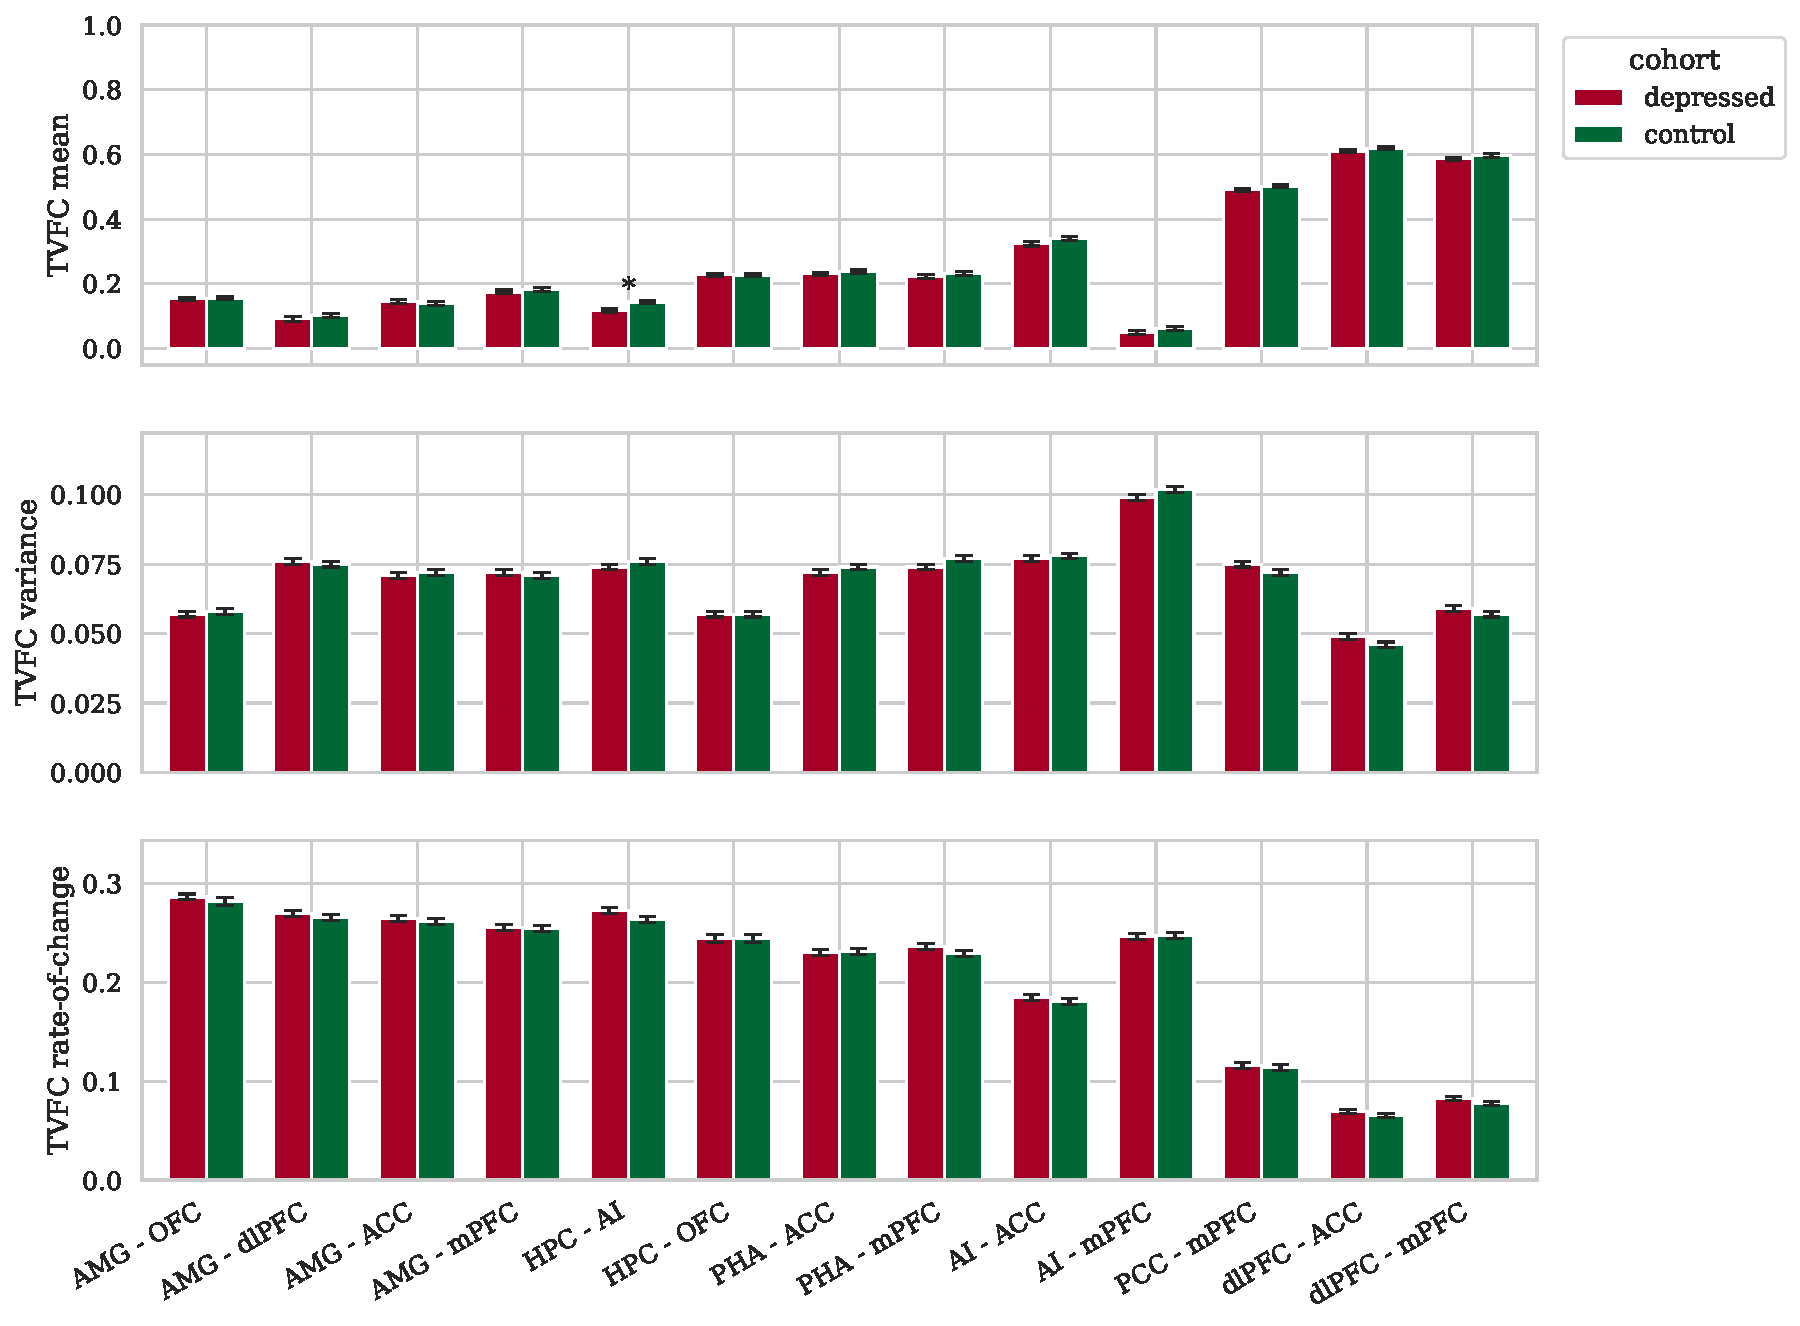
\includegraphics[width=\textwidth]{fig/ukbiobank/TVFC_predictions_summaries/lifetime_occurrence/cohort_comparison/ROI/correlation_all_TVFC_summary_measures_SW_cross_validated_edges_of_interest}
    \caption{
        Self-reported depression lifetime occurrence analysis - brain regions of interest - SW-CV estimates.
        Mean and standard error over 808 subjects per cohort for edges of interest for three TVFC summary measures.
        *: $p \leq .05$.
    }\label{fig:ukb-results-lo-roi-cohort-comparison-edges-of-interest-sw-cv}
\end{figure}


\begin{figure}[h]
    \centering
    \includegraphics[width=\textwidth]{fig/ukbiobank/TVFC_predictions_summaries/lifetime_occurrence/cohort_comparison/ROI/correlation_all_TVFC_summary_measures_SW_30_edges_of_interest}
    \caption{
        Self-reported depression lifetime occurrence analysis - brain regions of interest - SW (30 seconds window) estimates.
        Mean and standard error over 808 subjects per cohort for edges of interest for three TVFC summary measures.
        *: $p \leq .05$.
    }\label{fig:ukb-results-lo-roi-cohort-comparison-edges-of-interest-sw-30}
\end{figure}


\begin{figure}[h]
    \centering
    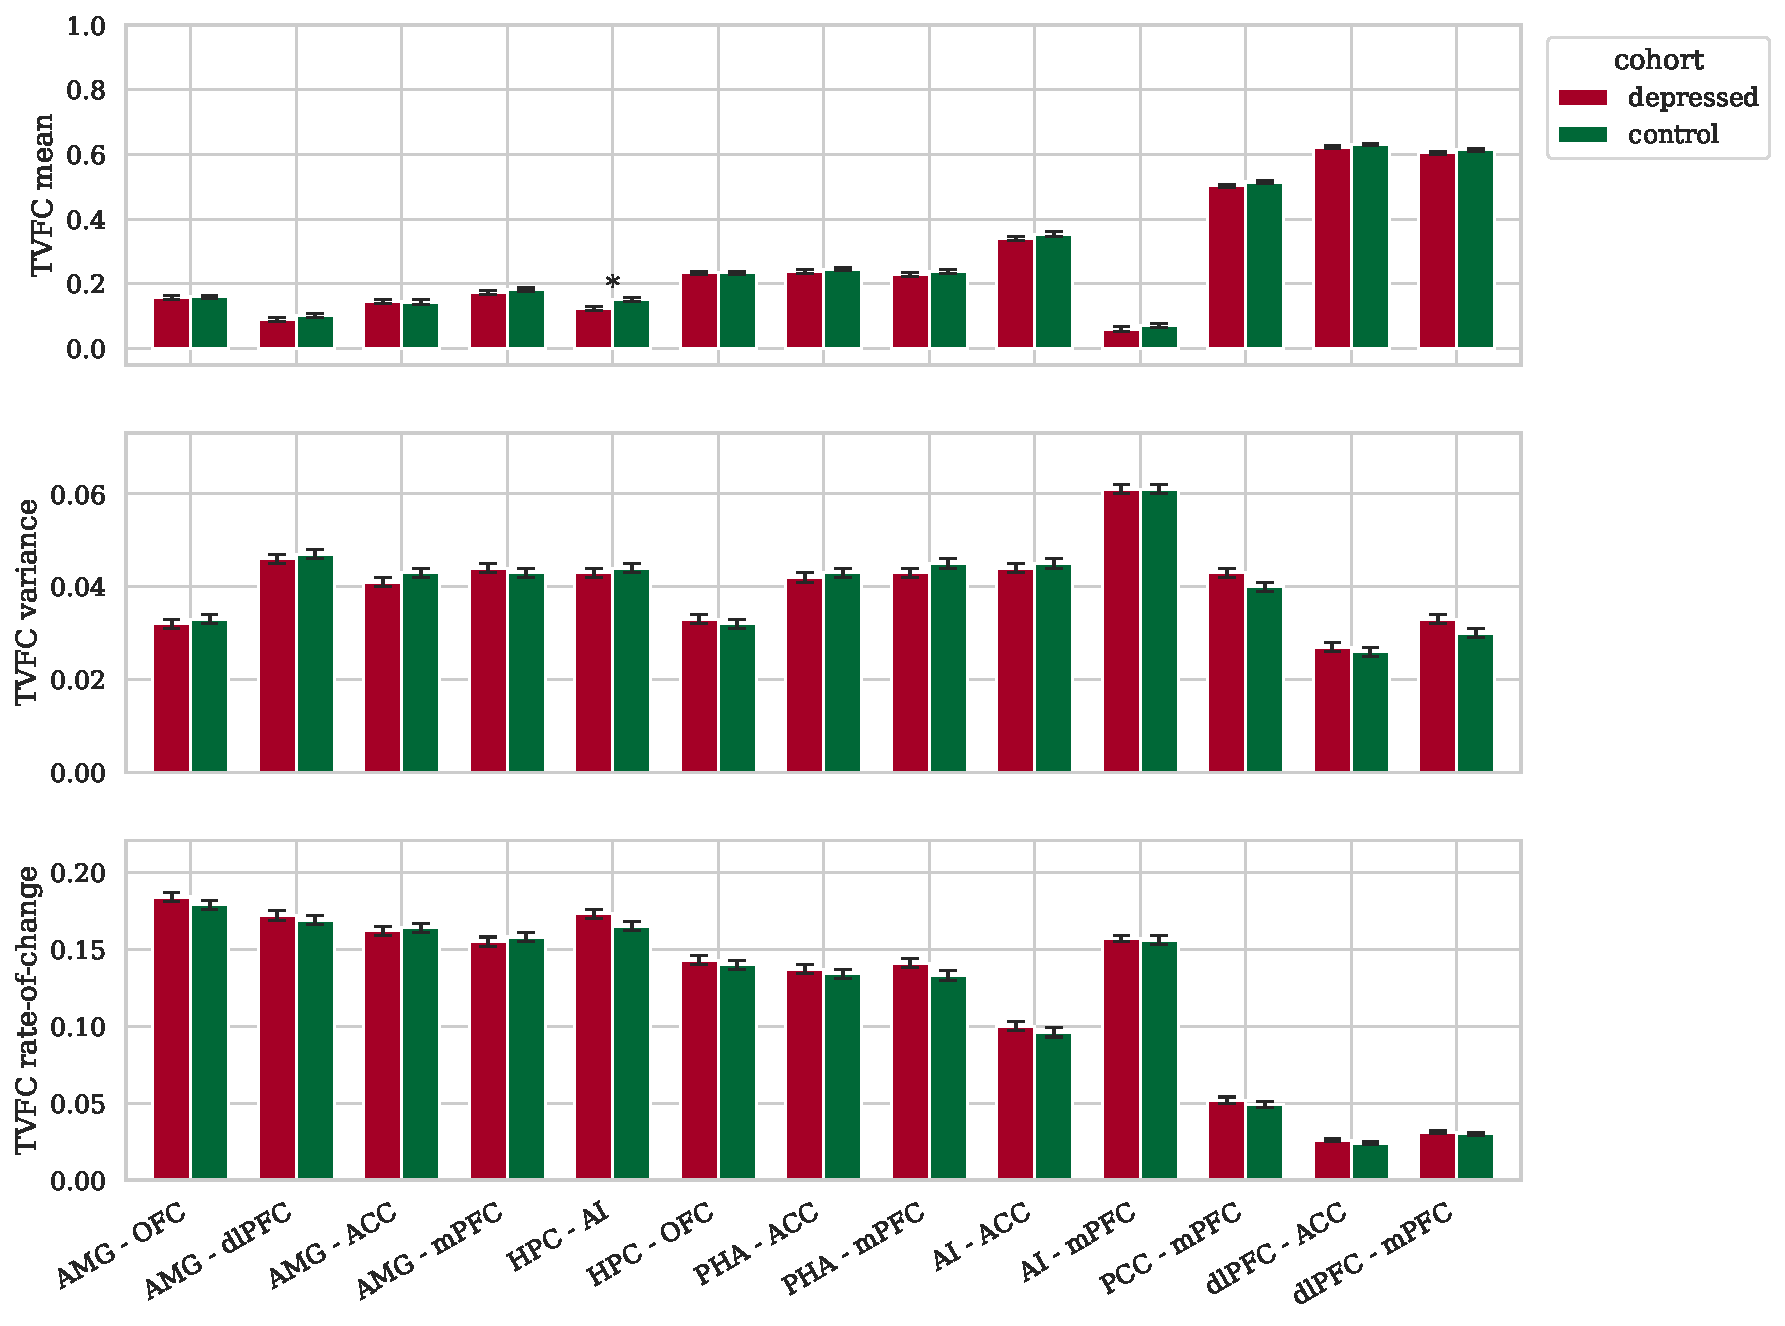
\includegraphics[width=\textwidth]{fig/ukbiobank/TVFC_predictions_summaries/lifetime_occurrence/cohort_comparison/ROI/correlation_all_TVFC_summary_measures_SW_60_edges_of_interest}
    \caption{
        Self-reported depression lifetime occurrence analysis - brain regions of interest - SW (60 seconds window) estimates.
        Mean and standard error over 808 subjects per cohort for edges of interest for three TVFC summary measures.
        *: $p \leq .05$.
    }\label{fig:ukb-results-lo-roi-cohort-comparison-edges-of-interest-sw-60}
\end{figure}


%%
\clearpage
\subsection{Self-reported lifetime occurrence - FN analysis}
%%


\begin{figure}[h]
    \centering
    \includegraphics[width=0.7\textwidth]{fig/ukbiobank/TVFC_predictions_summaries/lifetime_occurrence/cohort_comparison/FN/correlation_all_TVFC_summary_measures_DCC_joint_edges_of_interest}
    \caption{
        Self-reported depression lifetime occurrence analysis - functional networks - DCC (joint) estimates.
        Mean and standard error over 808 subjects per cohort for edges of interest for three TVFC summary measures.
        *: $p \leq .05$.
    }\label{fig:ukb-results-lo-fn-cohort-comparison-edges-of-interest-dcc-j}
\end{figure}


\begin{figure}[h]
    \centering
    \includegraphics[width=0.7\textwidth]{fig/ukbiobank/TVFC_predictions_summaries/lifetime_occurrence/cohort_comparison/FN/correlation_all_TVFC_summary_measures_DCC_bivariate_loop_edges_of_interest}
    \caption{
        Self-reported depression lifetime occurrence analysis - functional networks - DCC (bivariate loop) estimates.
        Mean and standard error over 808 subjects per cohort for edges of interest for three TVFC summary measures.
        *: $p \leq .05$.
    }\label{fig:ukb-results-lo-fn-cohort-comparison-edges-of-interest-dcc-bl}
\end{figure}


\begin{figure}[h]
    \centering
    \includegraphics[width=0.7\textwidth]{fig/ukbiobank/TVFC_predictions_summaries/lifetime_occurrence/cohort_comparison/FN/correlation_all_TVFC_summary_measures_SW_cross_validated_edges_of_interest}
    \caption{
        Self-reported depression lifetime occurrence analysis - functional networks - SW-CV estimates.
        Mean and standard error over 808 subjects per cohort for edges of interest for three TVFC summary measures.
        *: $p \leq .05$.
    }\label{fig:ukb-results-lo-fn-cohort-comparison-edges-of-interest-sw-cv}
\end{figure}


\begin{figure}[h]
    \centering
    \includegraphics[width=0.7\textwidth]{fig/ukbiobank/TVFC_predictions_summaries/lifetime_occurrence/cohort_comparison/FN/correlation_all_TVFC_summary_measures_SW_30_edges_of_interest}
    \caption{
        Self-reported depression lifetime occurrence analysis - functional networks - SW (30 seconds window) estimates.
        Mean and standard error over 808 subjects per cohort for edges of interest for three TVFC summary measures.
        *: $p \leq .05$.
    }\label{fig:ukb-results-lo-fn-cohort-comparison-edges-of-interest-sw-30}
\end{figure}


\begin{figure}[h]
    \centering
    \includegraphics[width=0.7\textwidth]{fig/ukbiobank/TVFC_predictions_summaries/lifetime_occurrence/cohort_comparison/FN/correlation_all_TVFC_summary_measures_SW_60_edges_of_interest}
    \caption{
        Self-reported depression lifetime occurrence analysis - functional networks - SW (60 seconds window) estimates.
        Mean and standard error over 808 subjects per cohort for edges of interest for three TVFC summary measures.
        *: $p \leq .05$.
    }\label{fig:ukb-results-lo-fn-cohort-comparison-edges-of-interest-sw-60}
\end{figure}



%%%%%%%%%%%%%%%%%%%%%%%%%%%%%%%%%%%%%%%%%%%%%%%%%%%%%%
%%%%%%%%%%%%%%%%%%%%%%%%%%%%%%%%%%%%%%%%%%%%%%%%%%%%%%
%%%%%%%%%%%%%%%%%%%%%%%%%%%%%%%%%%%%%%%%%%%%%%%%%%%%%%
%%%%%%%%%%%%%%%%%%%%%%%%%%%%%%%%%%%%%%%%%%%%%%%%%%%%%%
%%%%%%%%%%%%%%%%%%%%%%%%%%%%%%%%%%%%%%%%%%%%%%%%%%%%%%



%%
\clearpage
\subsection{Self-reported depressed state - ROI analysis}
%%


\begin{figure}[h]
  \centering
  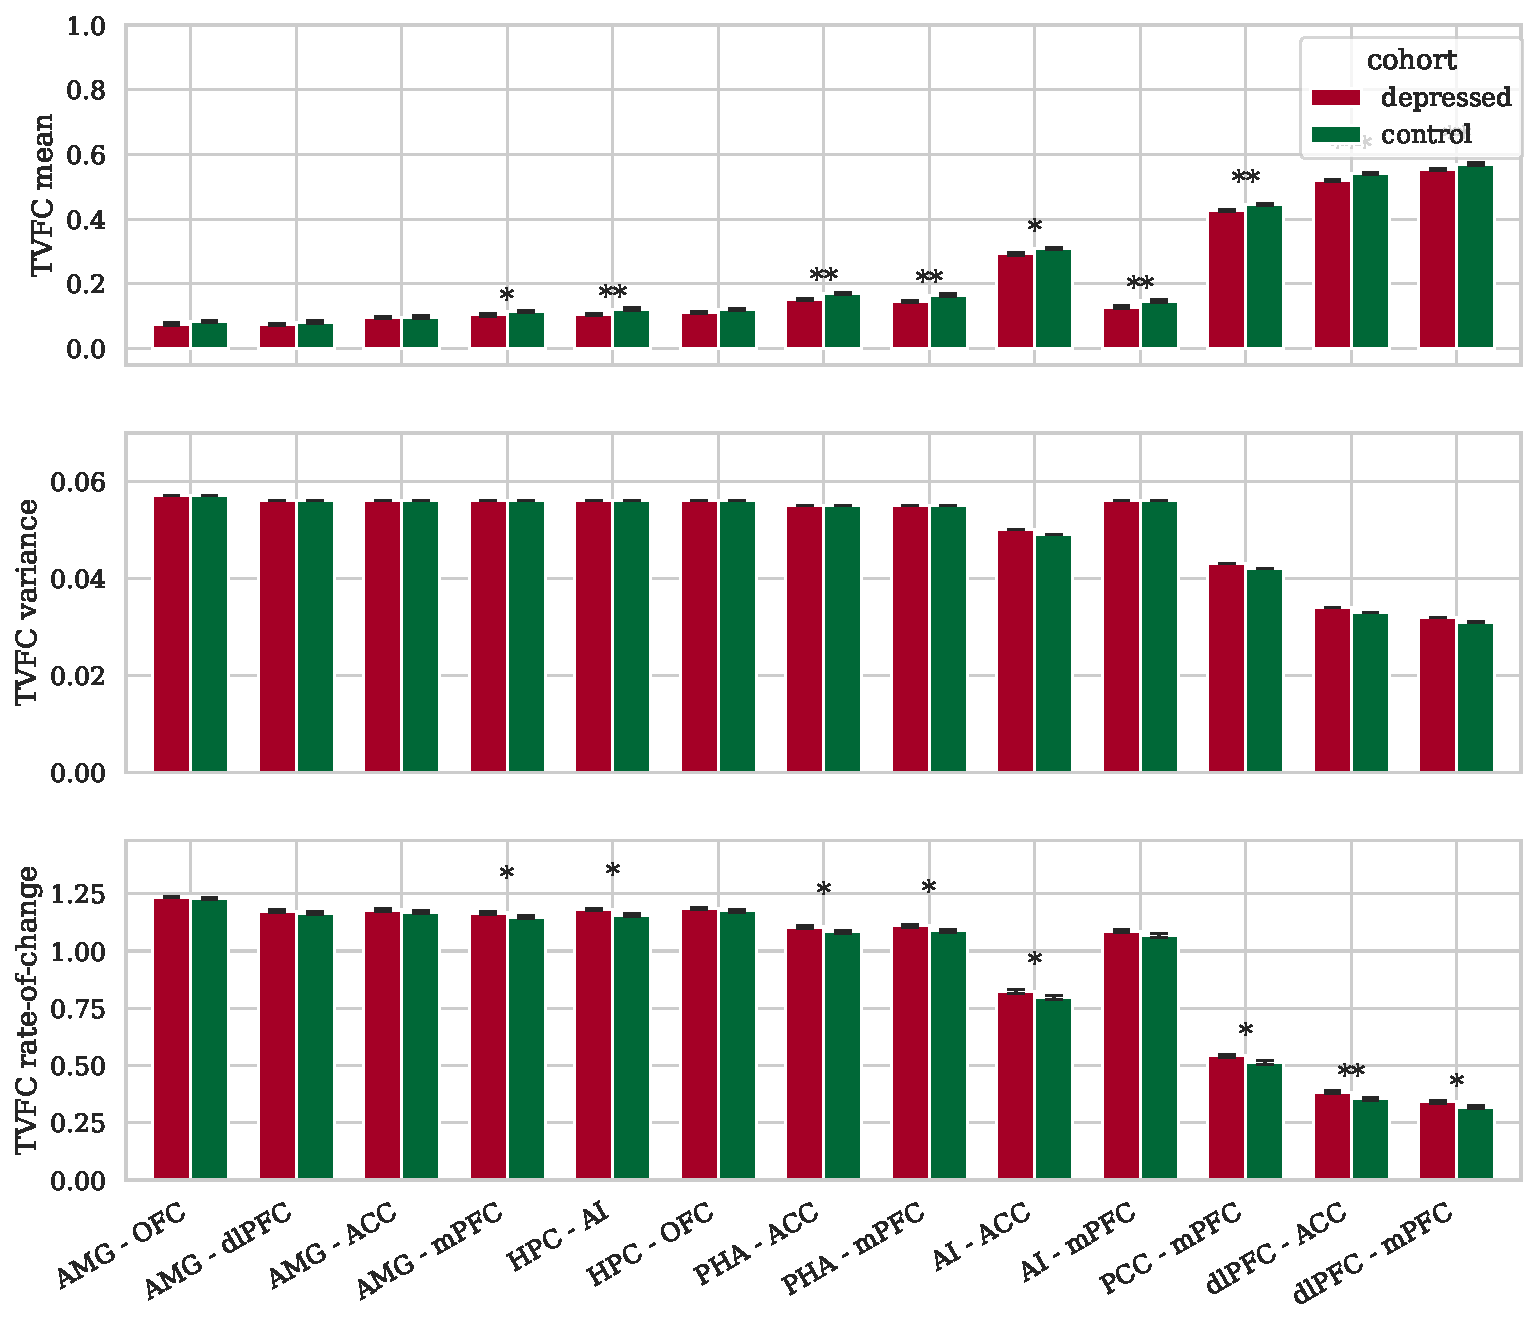
\includegraphics[width=\textwidth]{fig/ukbiobank/TVFC_predictions_summaries/self_reported_depression_state/cohort_comparison/ROI/correlation_all_TVFC_summary_measures_DCC_joint_edges_of_interest}
  \caption{
    Self-reported depressed state analysis - brain regions of interest - DCC (joint) estimates.
    Mean and standard error over 1,411 subjects per cohort for edges of interest for three TVFC summary measures.
    *: $p \leq .05$, **: $p \leq .01$, ***: $p \leq .001$.
  }\label{fig:ukb-results-srds-roi-cohort-comparison-edges-of-interest-dcc-j}
\end{figure}


\begin{figure}[h]
    \centering
    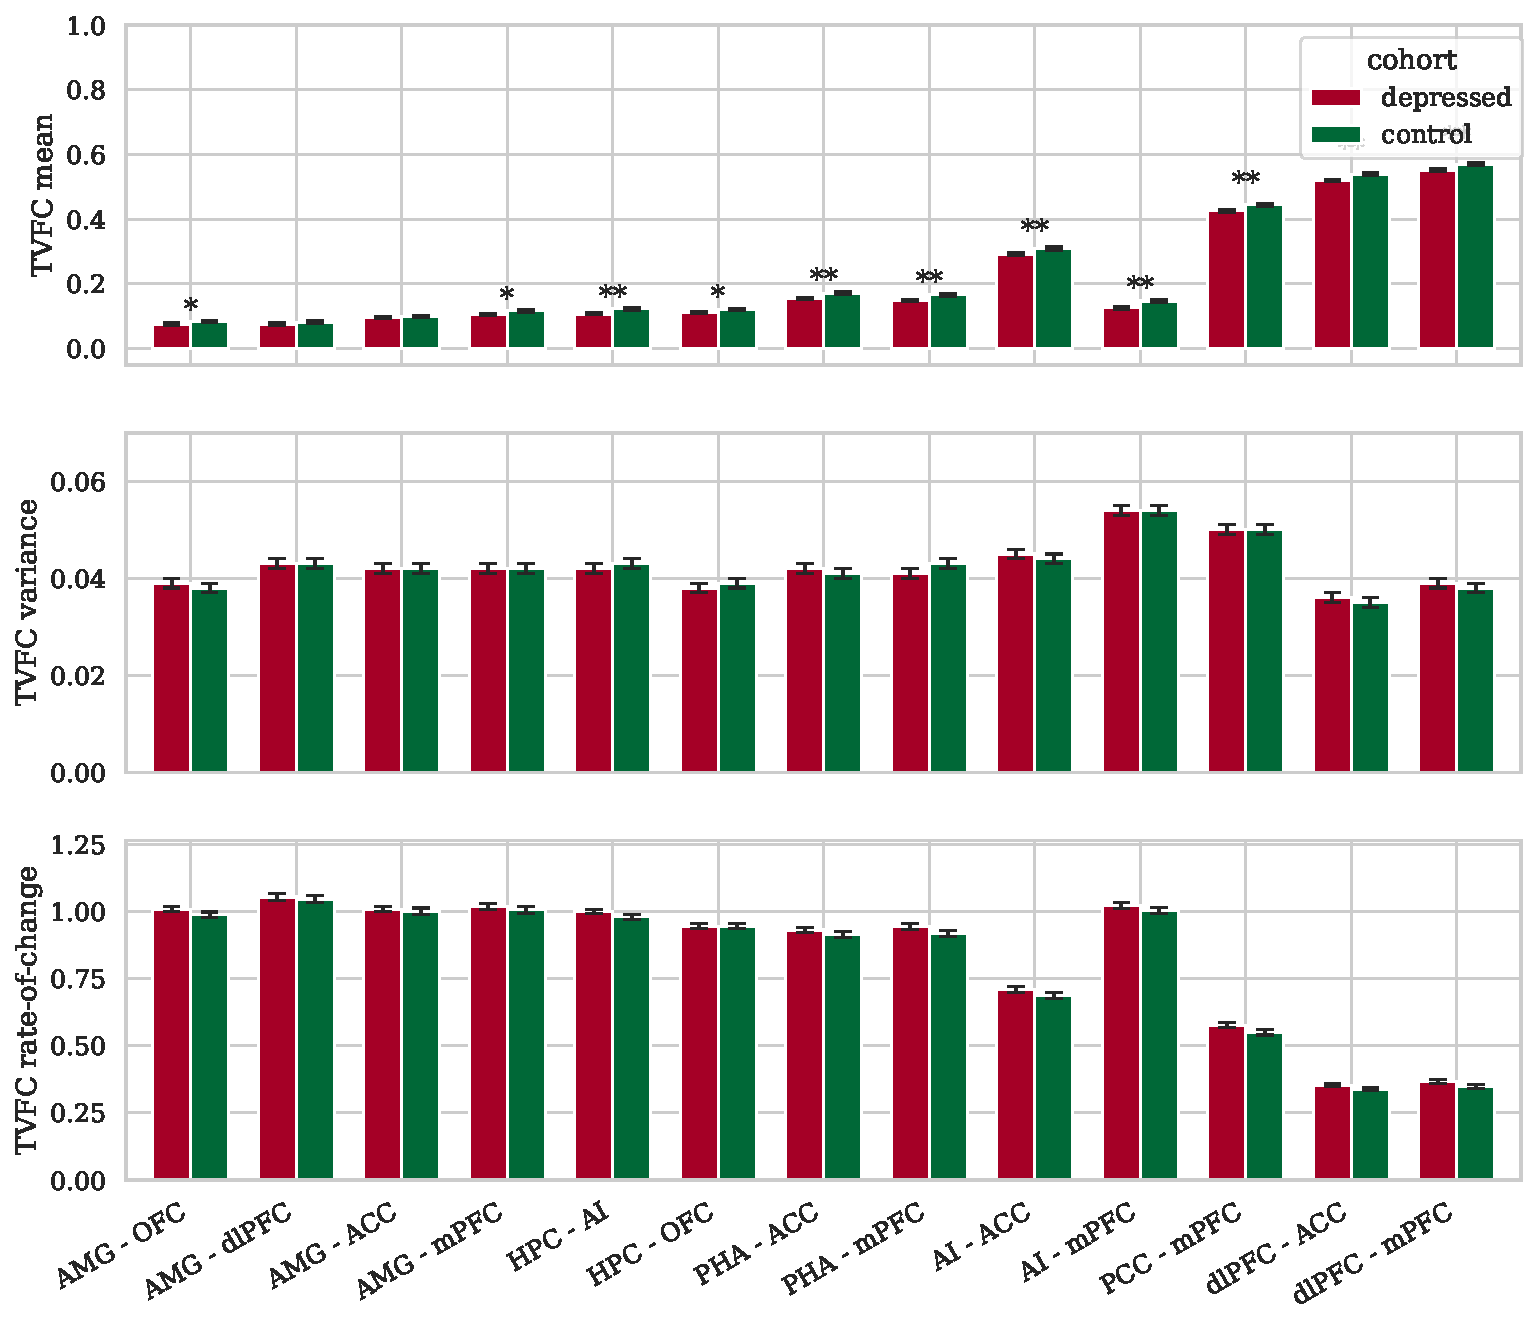
\includegraphics[width=\textwidth]{fig/ukbiobank/TVFC_predictions_summaries/self_reported_depression_state/cohort_comparison/ROI/correlation_all_TVFC_summary_measures_DCC_bivariate_loop_edges_of_interest}
    \caption{
        Self-reported depressed state analysis - brain regions of interest - DCC (bivariate loop) estimates.
        Mean and standard error over 1,411 subjects per cohort for edges of interest for three TVFC summary measures.
        *: $p \leq .05$, **: $p \leq .01$, ***: $p \leq .001$.
    }\label{fig:ukb-results-srds-roi-cohort-comparison-edges-of-interest-dcc-bl}
\end{figure}


\begin{figure}[h]
  \centering
  \includegraphics[width=\textwidth]{fig/ukbiobank/TVFC_predictions_summaries/self_reported_depression_state/cohort_comparison/ROI/correlation_all_TVFC_summary_measures_SW_cross_validated_edges_of_interest}
  \caption{
    Self-reported depressed state analysis - brain regions of interest - SW-CV estimates.
    Mean and standard error over 1,411 subjects per cohort for edges of interest for three TVFC summary measures.
    *: $p \leq .05$, **: $p \leq .01$, ***: $p \leq .001$.
  }\label{fig:ukb-results-srds-roi-cohort-comparison-edges-of-interest-sw-cv}
\end{figure}


\begin{figure}[h]
    \centering
    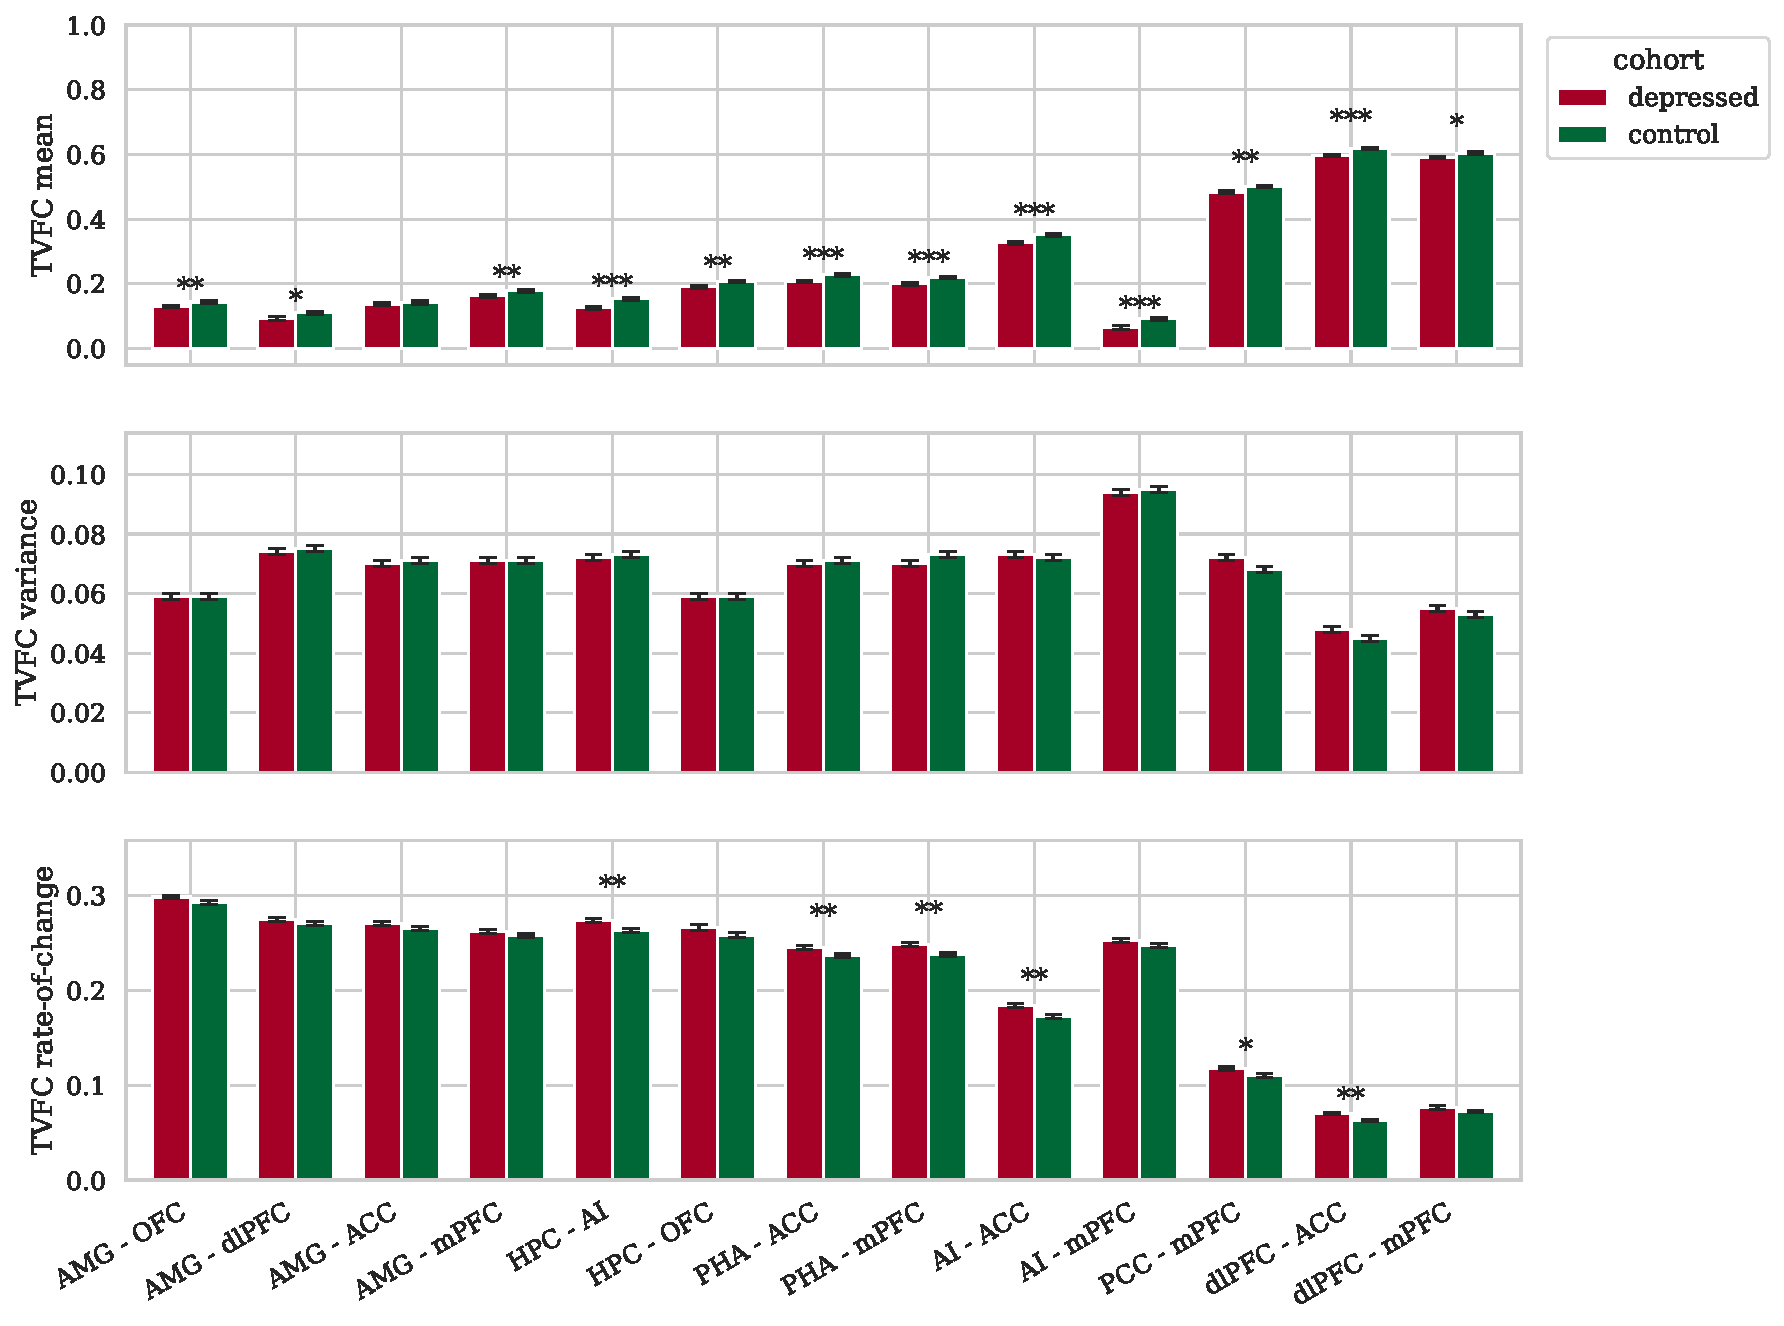
\includegraphics[width=\textwidth]{fig/ukbiobank/TVFC_predictions_summaries/self_reported_depression_state/cohort_comparison/ROI/correlation_all_TVFC_summary_measures_SW_30_edges_of_interest}
    \caption{
        Self-reported depressed state analysis - brain regions of interest - SW (30 seconds window) estimates.
        Mean and standard error over 1,411 subjects per cohort for edges of interest for three TVFC summary measures.
        *: $p \leq .05$, **: $p \leq .01$, ***: $p \leq .001$.
    }\label{fig:ukb-results-srds-roi-cohort-comparison-edges-of-interest-sw-30}
\end{figure}


\begin{figure}[h]
    \centering
    \includegraphics[width=\textwidth]{fig/ukbiobank/TVFC_predictions_summaries/self_reported_depression_state/cohort_comparison/ROI/correlation_all_TVFC_summary_measures_SW_60_edges_of_interest}
    \caption{
        Self-reported depressed state analysis - brain regions of interest - SW (60 seconds window) estimates.
        Mean and standard error over 1,411 subjects per cohort for edges of interest for three TVFC summary measures.
        *: $p \leq .05$, **: $p \leq .01$, ***: $p \leq .001$.
    }\label{fig:ukb-results-srds-roi-cohort-comparison-edges-of-interest-sw-60}
\end{figure}


%%
\clearpage
\subsection{Self-reported depressed state - FN analysis}
%%


\begin{figure}[h]
    \centering
    \includegraphics[width=0.7\textwidth]{fig/ukbiobank/TVFC_predictions_summaries/self_reported_depression_state/cohort_comparison/FN/correlation_all_TVFC_summary_measures_DCC_joint_edges_of_interest}
    \caption{
        Self-reported depressed state analysis - functional networks - DCC (joint) estimates.
        Mean and standard error over 1,411 subjects per cohort for edges of interest for three TVFC summary measures.
        *: $p \leq .05$, **: $p \leq .01$, ***: $p \leq .001$.
    }\label{fig:ukb-results-srds-fn-cohort-comparison-edges-of-interest-dcc-j}
\end{figure}


\begin{figure}[h]
    \centering
    \includegraphics[width=0.7\textwidth]{fig/ukbiobank/TVFC_predictions_summaries/self_reported_depression_state/cohort_comparison/FN/correlation_all_TVFC_summary_measures_DCC_bivariate_loop_edges_of_interest}
    \caption{
        Self-reported depressed state analysis - functional networks - DCC (bivariate loop) estimates.
        Mean and standard error over 1,411 subjects per cohort for edges of interest for three TVFC summary measures.
        *: $p \leq .05$, **: $p \leq .01$, ***: $p \leq .001$.
    }\label{fig:ukb-results-srds-fn-cohort-comparison-edges-of-interest-dcc-bl}
\end{figure}


\begin{figure}[h]
    \centering
    \includegraphics[width=0.7\textwidth]{fig/ukbiobank/TVFC_predictions_summaries/self_reported_depression_state/cohort_comparison/FN/correlation_all_TVFC_summary_measures_SW_cross_validated_edges_of_interest}
    \caption{
        Self-reported depressed state analysis - functional networks - SW-CV estimates.
        Mean and standard error over 1,411 subjects per cohort for edges of interest for three TVFC summary measures.
        *: $p \leq .05$, **: $p \leq .01$, ***: $p \leq .001$.
    }\label{fig:ukb-results-srds-fn-cohort-comparison-edges-of-interest-sw-cv}
\end{figure}


\begin{figure}[h]
    \centering
    \includegraphics[width=0.7\textwidth]{fig/ukbiobank/TVFC_predictions_summaries/self_reported_depression_state/cohort_comparison/FN/correlation_all_TVFC_summary_measures_SW_30_edges_of_interest}
    \caption{
        Self-reported depressed state analysis - functional networks - SW (30 seconds window) estimates.
        Mean and standard error over 1,411 subjects per cohort for edges of interest for three TVFC summary measures.
        *: $p \leq .05$, **: $p \leq .01$, ***: $p \leq .001$.
    }\label{fig:ukb-results-srds-fn-cohort-comparison-edges-of-interest-sw-30}
\end{figure}


\begin{figure}[h]
  \centering
  \includegraphics[width=0.7\textwidth]{fig/ukbiobank/TVFC_predictions_summaries/self_reported_depression_state/cohort_comparison/FN/correlation_all_TVFC_summary_measures_SW_60_edges_of_interest}
  \caption{
    Self-reported depressed state analysis - functional networks - SW (60 seconds window) estimates.
    Mean and standard error over 1,411 subjects per cohort for edges of interest for three TVFC summary measures.
    *: $p \leq .05$, **: $p \leq .01$, ***: $p \leq .001$.
  }\label{fig:ukb-results-srds-fn-cohort-comparison-edges-of-interest-sw-60}
\end{figure}



%%%%%%%%%%%%%%%%%%%%%%%%%%%%%%%%%%%%%%%%%%%%%%%%%%%%%%
%%%%%%%%%%%%%%%%%%%%%%%%%%%%%%%%%%%%%%%%%%%%%%%%%%%%%%
%%%%%%%%%%%%%%%%%%%%%%%%%%%%%%%%%%%%%%%%%%%%%%%%%%%%%%
%%%%%%%%%%%%%%%%%%%%%%%%%%%%%%%%%%%%%%%%%%%%%%%%%%%%%%
%%%%%%%%%%%%%%%%%%%%%%%%%%%%%%%%%%%%%%%%%%%%%%%%%%%%%%



%%
\clearpage
\subsection{Polygenic risk scores - ROI analysis}
%%


\begin{figure}[h]
    \centering
    \includegraphics[width=\textwidth]{fig/ukbiobank/TVFC_predictions_summaries/pgs/cohort_comparison/ROI/correlation_all_TVFC_summary_measures_DCC_joint_edges_of_interest}
    \caption{
        Polygenic risk scores analysis - brain regions of interest - DCC (joint) estimates.
        Mean and standard error over 3,775 subjects per cohort for edges of interest for three TVFC summary measures.
    }\label{fig:ukb-results-pgs-roi-cohort-comparison-edges-of-interest-dcc-j}
\end{figure}


\begin{figure}[h]
    \centering
    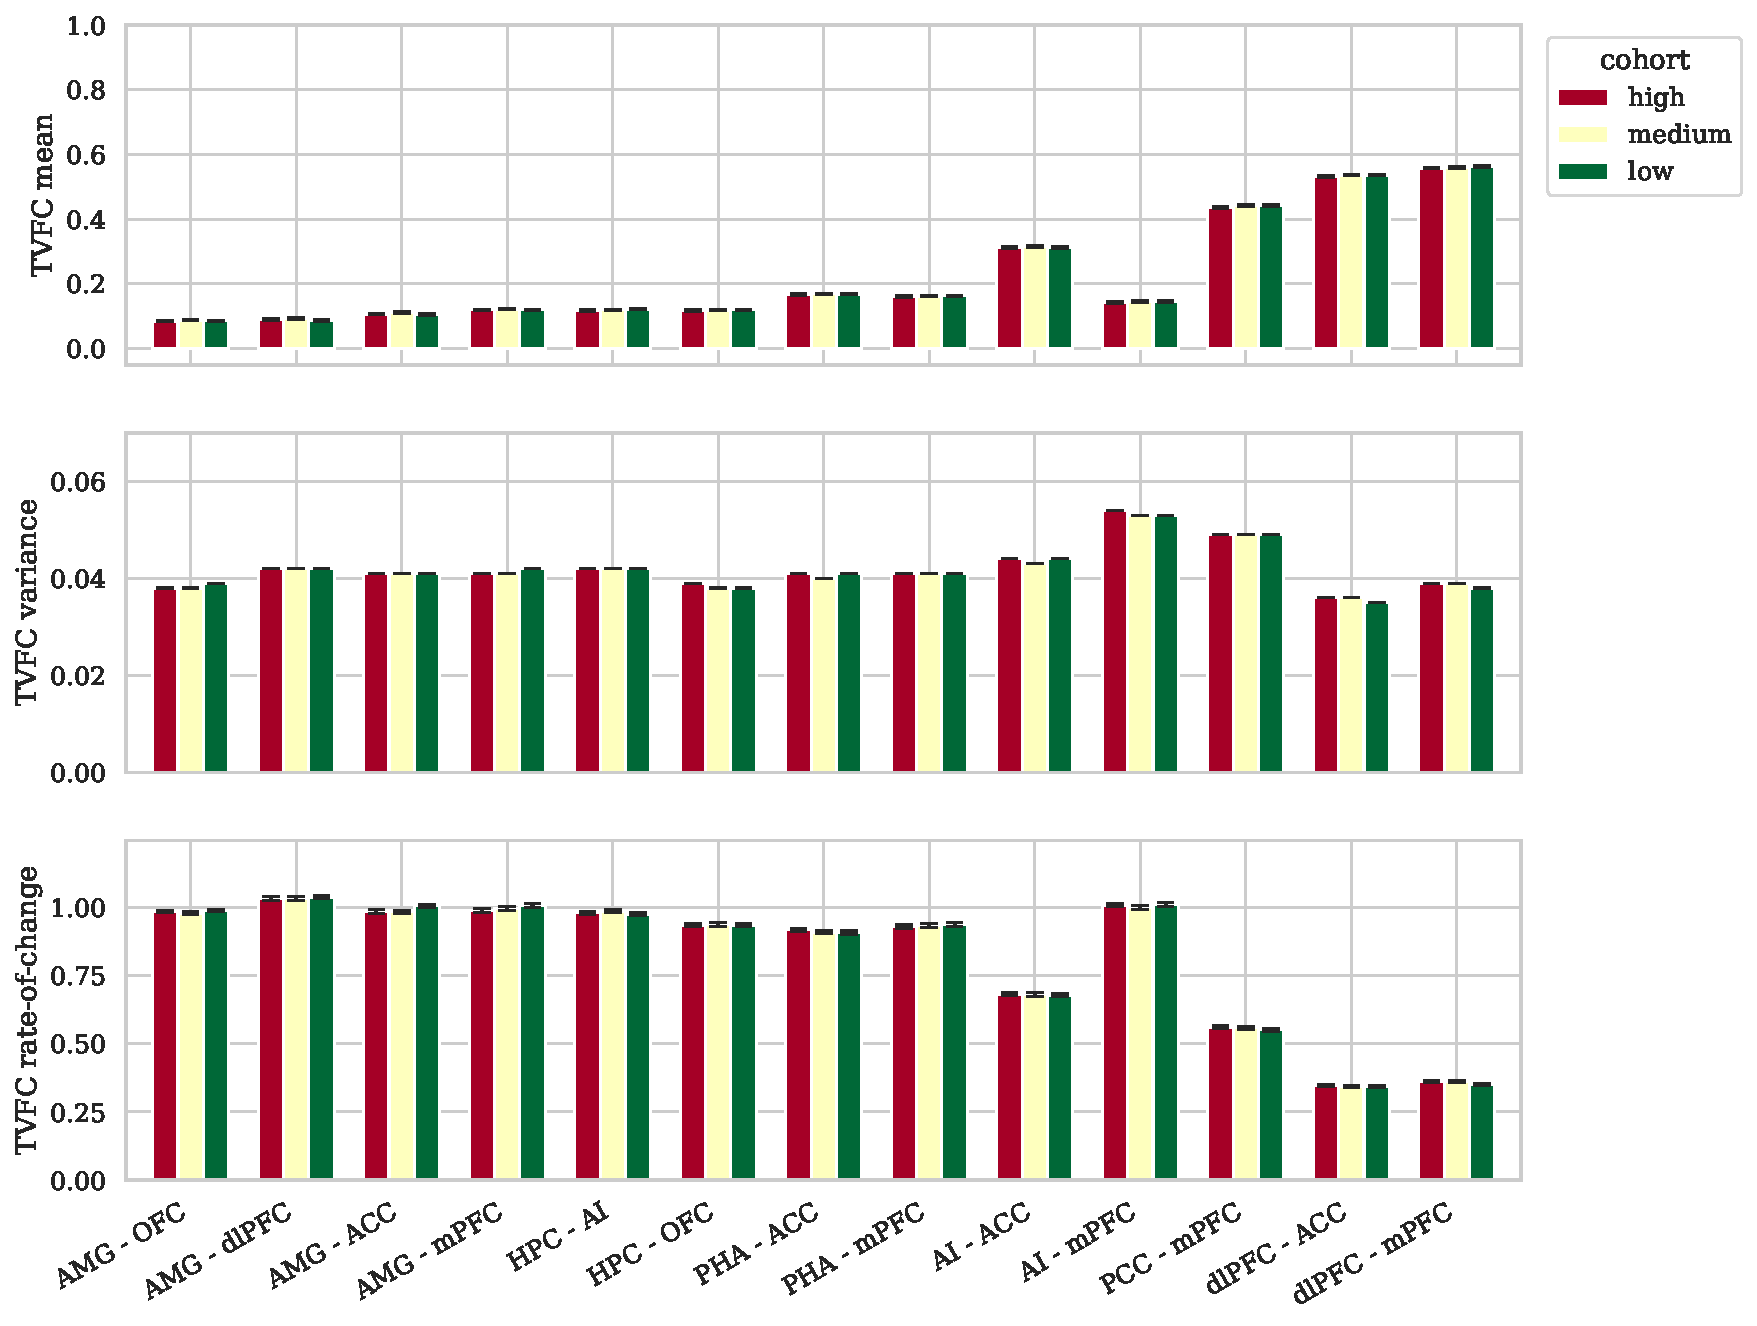
\includegraphics[width=\textwidth]{fig/ukbiobank/TVFC_predictions_summaries/pgs/cohort_comparison/ROI/correlation_all_TVFC_summary_measures_DCC_bivariate_loop_edges_of_interest}
    \caption{
        Polygenic risk scores analysis - brain regions of interest - DCC (bivariate loop) estimates.
        Mean and standard error over 3,775 subjects per cohort for edges of interest for three TVFC summary measures.
    }\label{fig:ukb-results-pgs-roi-cohort-comparison-edges-of-interest-dcc-bl}
\end{figure}


\begin{figure}[h]
    \centering
    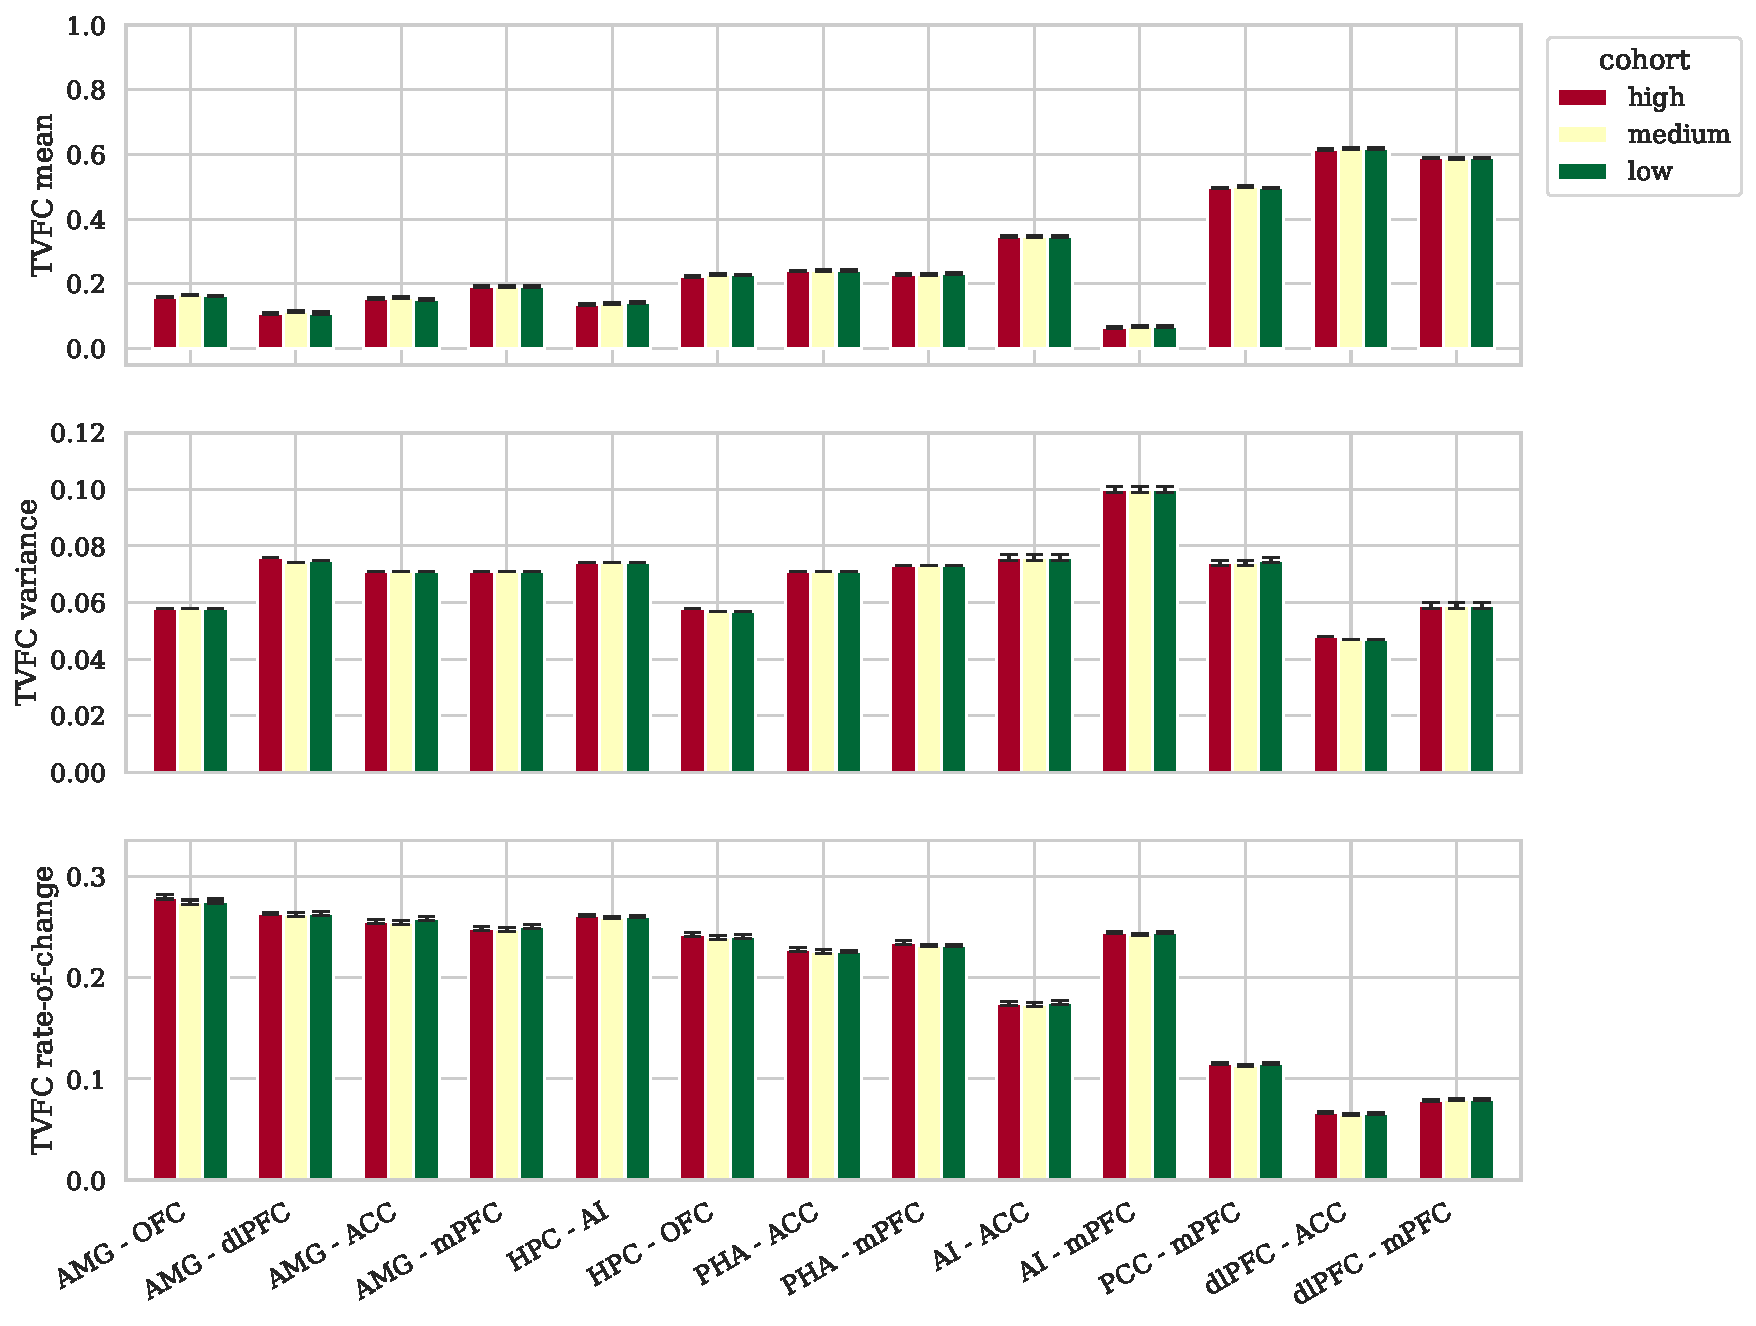
\includegraphics[width=\textwidth]{fig/ukbiobank/TVFC_predictions_summaries/pgs/cohort_comparison/ROI/correlation_all_TVFC_summary_measures_SW_cross_validated_edges_of_interest}
    \caption{
        Polygenic risk scores analysis - brain regions of interest - SW-CV estimates.
        Mean and standard error over 3,775 subjects per cohort for edges of interest for three TVFC summary measures.
    }\label{fig:ukb-results-pgs-roi-cohort-comparison-edges-of-interest-sw-cv}
\end{figure}


\begin{figure}[h]
    \centering
    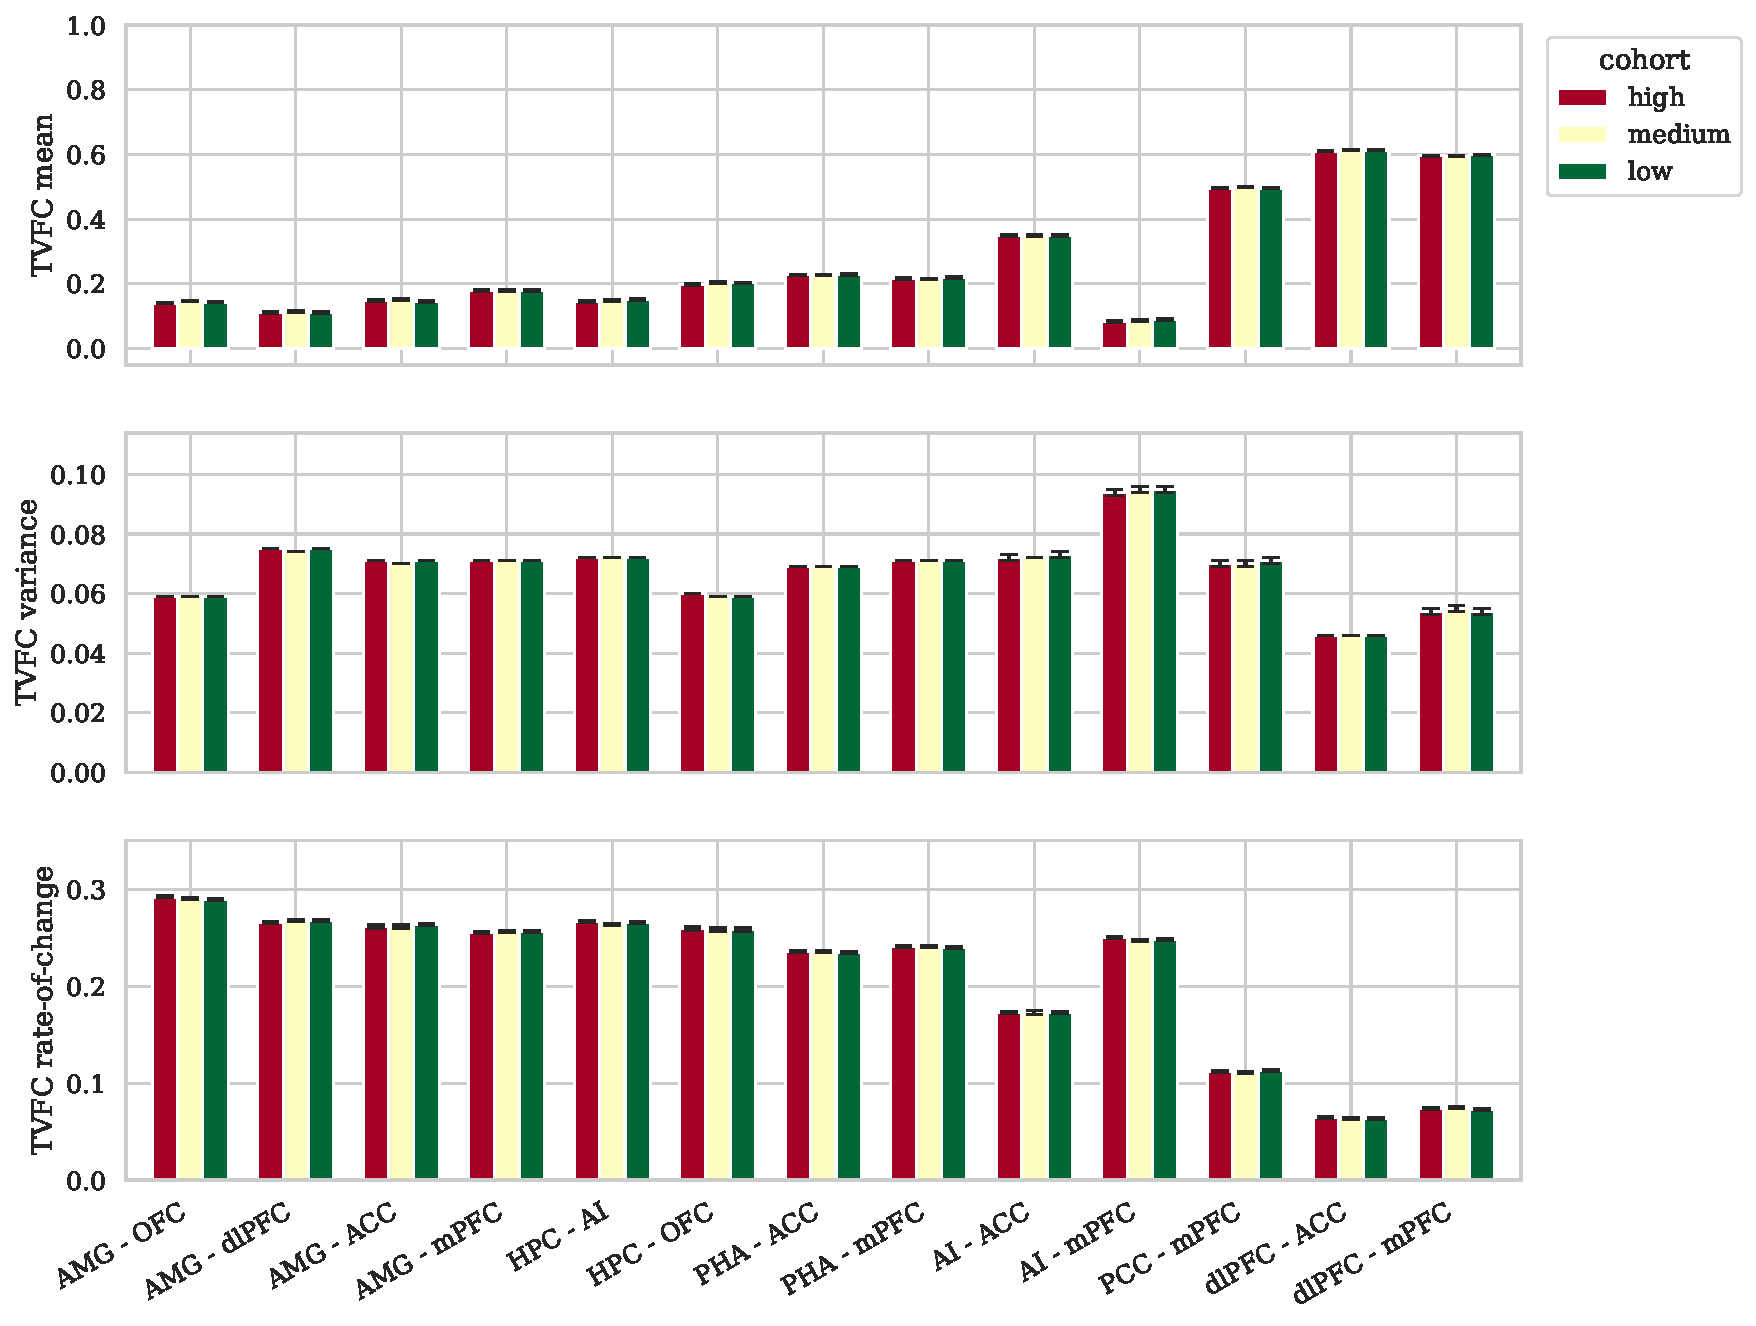
\includegraphics[width=\textwidth]{fig/ukbiobank/TVFC_predictions_summaries/pgs/cohort_comparison/ROI/correlation_all_TVFC_summary_measures_SW_30_edges_of_interest}
    \caption{
        Polygenic risk scores analysis - brain regions of interest - SW (30 seconds window) estimates.
        Mean and standard error over 3,775 subjects per cohort for edges of interest for three TVFC summary measures.
    }\label{fig:ukb-results-pgs-roi-cohort-comparison-edges-of-interest-sw-30}
\end{figure}


\begin{figure}[h]
    \centering
    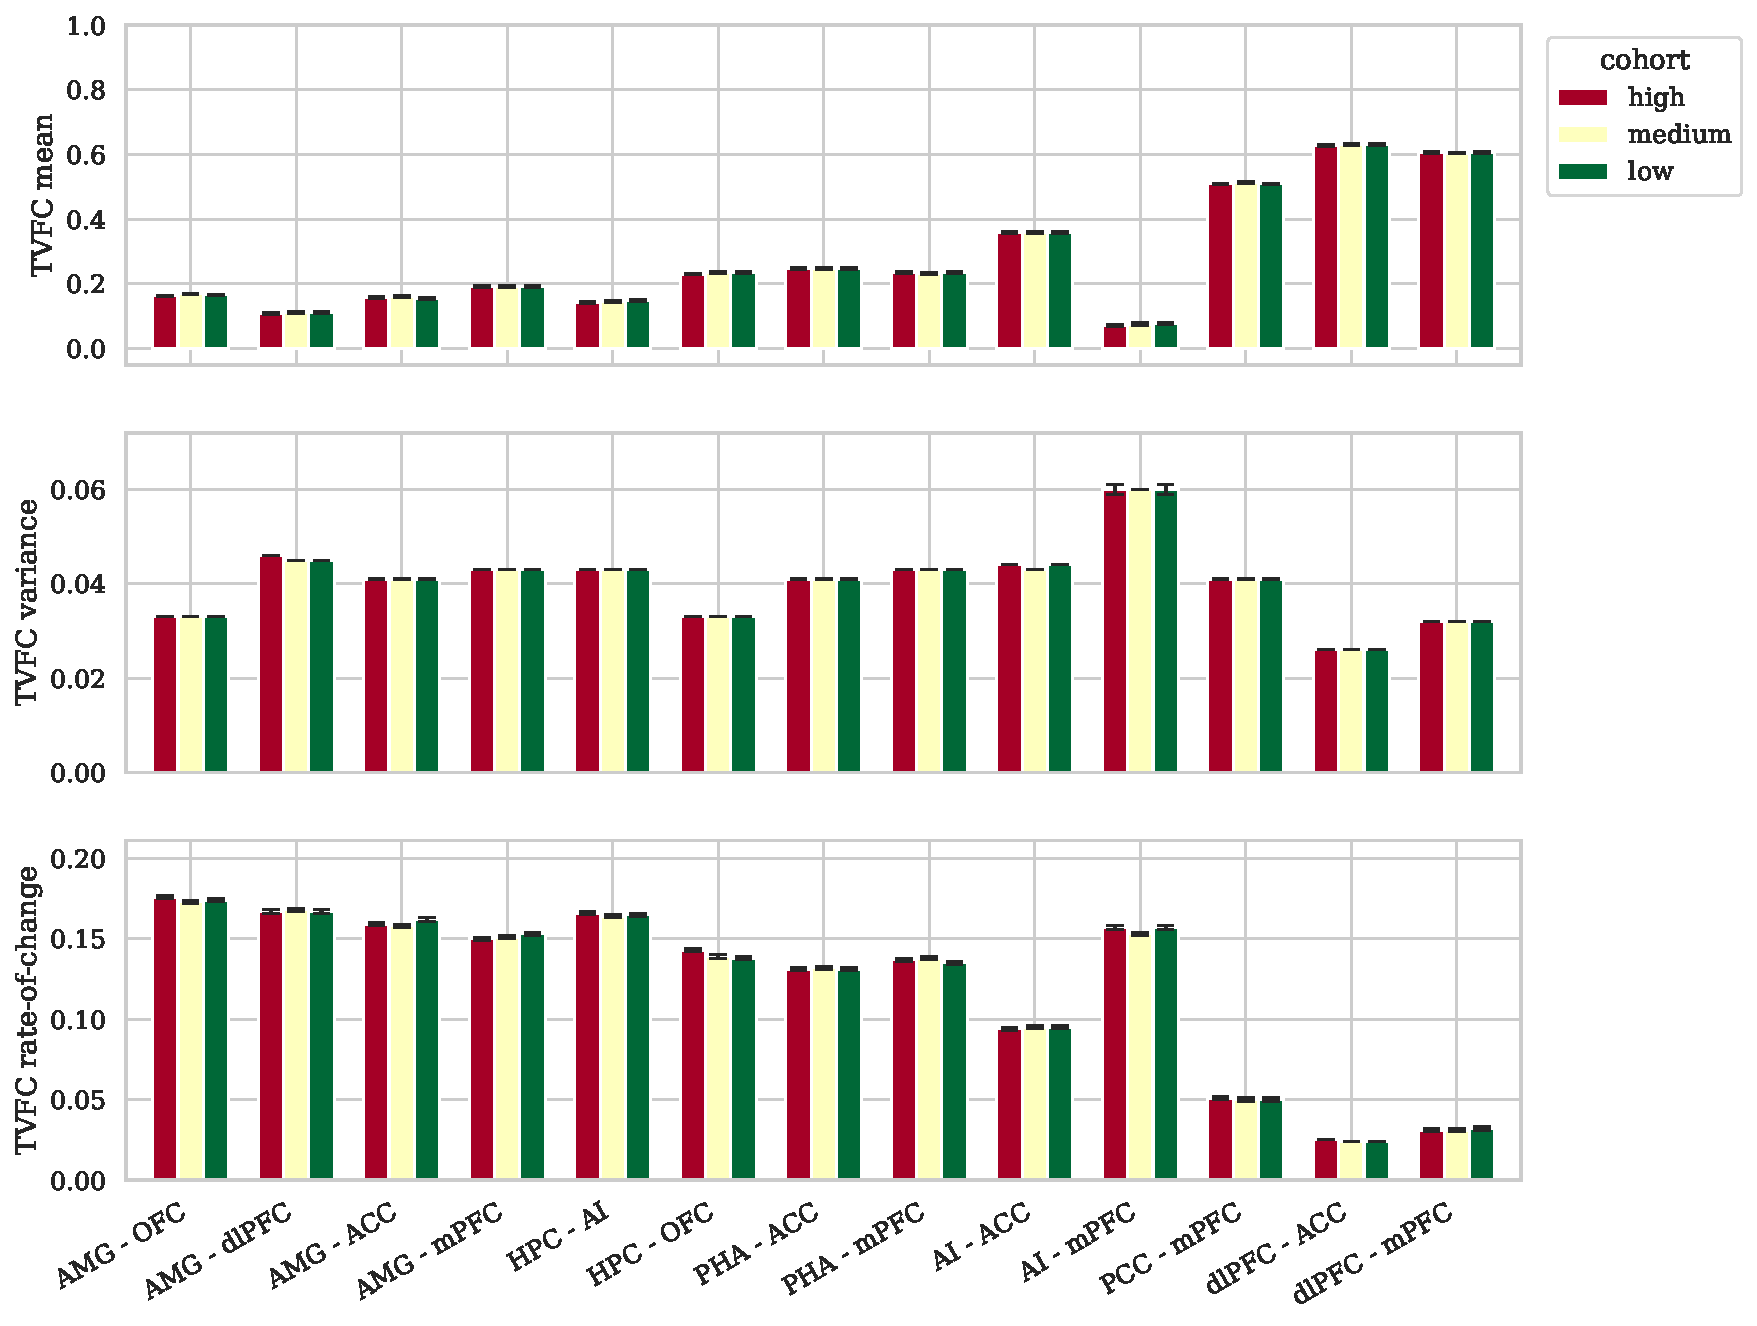
\includegraphics[width=\textwidth]{fig/ukbiobank/TVFC_predictions_summaries/pgs/cohort_comparison/ROI/correlation_all_TVFC_summary_measures_SW_60_edges_of_interest}
    \caption{
        Polygenic risk scores analysis - brain regions of interest - SW (60 seconds window) estimates.
        Mean and standard error over 3,775 subjects per cohort for edges of interest for three TVFC summary measures.
    }\label{fig:ukb-results-pgs-roi-cohort-comparison-edges-of-interest-sw-60}
\end{figure}


%%
\clearpage
\subsection{Polygenic risk scores - FN analysis}
%%


\begin{figure}[h]
  \centering
  \includegraphics[width=0.7\textwidth]{fig/ukbiobank/TVFC_predictions_summaries/pgs/cohort_comparison/FN/correlation_all_TVFC_summary_measures_DCC_joint_edges_of_interest}
  \caption{
    Polygenic risk scores analysis - functional networks - DCC (joint) estimates.
    Mean and standard error over 3,775 subjects per cohort for edges of interest for three TVFC summary measures.
  }\label{fig:ukb-results-pgs-fn-cohort-comparison-edges-of-interest-dcc-j}
\end{figure}


\begin{figure}[h]
  \centering
  \includegraphics[width=0.7\textwidth]{fig/ukbiobank/TVFC_predictions_summaries/pgs/cohort_comparison/FN/correlation_all_TVFC_summary_measures_DCC_bivariate_loop_edges_of_interest}
  \caption{
    Polygenic risk scores analysis - functional networks - DCC (bivariate loop) estimates.
    Mean and standard error over 3,775 subjects per cohort for edges of interest for three TVFC summary measures.
  }\label{fig:ukb-results-pgs-fn-cohort-comparison-edges-of-interest-dcc-bl}
\end{figure}


\begin{figure}[h]
    \centering
    \includegraphics[width=0.7\textwidth]{fig/ukbiobank/TVFC_predictions_summaries/pgs/cohort_comparison/FN/correlation_all_TVFC_summary_measures_SW_cross_validated_edges_of_interest}
    \caption{
        Polygenic risk scores analysis - functional networks - SW-CV estimates.
        Mean and standard error over 3,775 subjects per cohort for edges of interest for three TVFC summary measures.
    }\label{fig:ukb-results-pgs-fn-cohort-comparison-edges-of-interest-sw-cv}
\end{figure}


\begin{figure}[h]
    \centering
    \includegraphics[width=0.7\textwidth]{fig/ukbiobank/TVFC_predictions_summaries/pgs/cohort_comparison/FN/correlation_all_TVFC_summary_measures_SW_30_edges_of_interest}
    \caption{
        Polygenic risk scores analysis - functional networks - SW (30 seconds window) estimates.
        Mean and standard error over 3,775 subjects per cohort for edges of interest for three TVFC summary measures.
    }\label{fig:ukb-results-pgs-fn-cohort-comparison-edges-of-interest-sw-30}
\end{figure}


\begin{figure}[h]
    \centering
    \includegraphics[width=0.7\textwidth]{fig/ukbiobank/TVFC_predictions_summaries/pgs/cohort_comparison/FN/correlation_all_TVFC_summary_measures_SW_60_edges_of_interest}
    \caption{
        Polygenic risk scores analysis - functional networks - SW (60 seconds window) estimates.
        Mean and standard error over 3,775 subjects per cohort for edges of interest for three TVFC summary measures.
    }\label{fig:ukb-results-pgs-fn-cohort-comparison-edges-of-interest-sw-60}
\end{figure}
